\documentclass{article} % For LaTeX2e
\usepackage{nips2015,times}
\usepackage{hyperref}
\usepackage{url}
\usepackage{graphicx}
\graphicspath{ {./assets/} }
\usepackage{biblatex}
\addbibresource{refs.bib}


\usepackage{float}
\usepackage[inline]{enumitem}
\usepackage{booktabs}
\usepackage{multirow}
\usepackage[center]{caption}
\usepackage{subcaption}

\title{CSE 546 Assignment 2 - Deep Q-Networks}


\author{
   Ijaj Ahmed \\
   Department of Computer Science\\
   University at Buffalo, SUNY\\
   Buffalo, NY 14260 \\
   \texttt{ijajahme@buffalo.edu}
   \And
   Mohammed Nasheed Yasin \\
   Department of Linguistics\\
   University at Buffalo, SUNY\\
   Buffalo, NY 14260 \\
   \texttt{m44@buffalo.edu}
}

% The \author macro works with any number of authors. There are two commands
% used to separate the names and addresses of multiple authors: \And and \AND.
%
% Using \And between authors leaves it to \LaTeX{} to determine where to break
% the lines. Using \AND forces a linebreak at that point. So, if \LaTeX{}
% puts 3 of 4 authors names on the first line, and the last on the second
% line, try using \AND instead of \And before the third author name.

\newcommand{\fix}{\marginpar{FIX}}
\newcommand{\new}{\marginpar{NEW}}

\nipsfinalcopy

\begin{document}


\maketitle

\begin{abstract}
    This report presents our experiments on a self-created \verb|GridWorld| environment and two additional environments, \verb|CartPole-v1| and \verb|LunarLander-v2|. These environments were selected from the \verb|ClassicalControl| and \verb|Box2D| collections in the Gymnasium library \cite{1606.01540}. We applied DQN and Double DQN to solve these environments and conducted a case study on the outcomes.
\end{abstract}

\section*{Environment Description}


\section{The Grid-world Environment}
\label{sec:definition}

There are certain features that are common to both the stocastic and deterministic environments.

\subsection*{Environmental Elements}
\begin{figure}[h]
    \begin{center}
        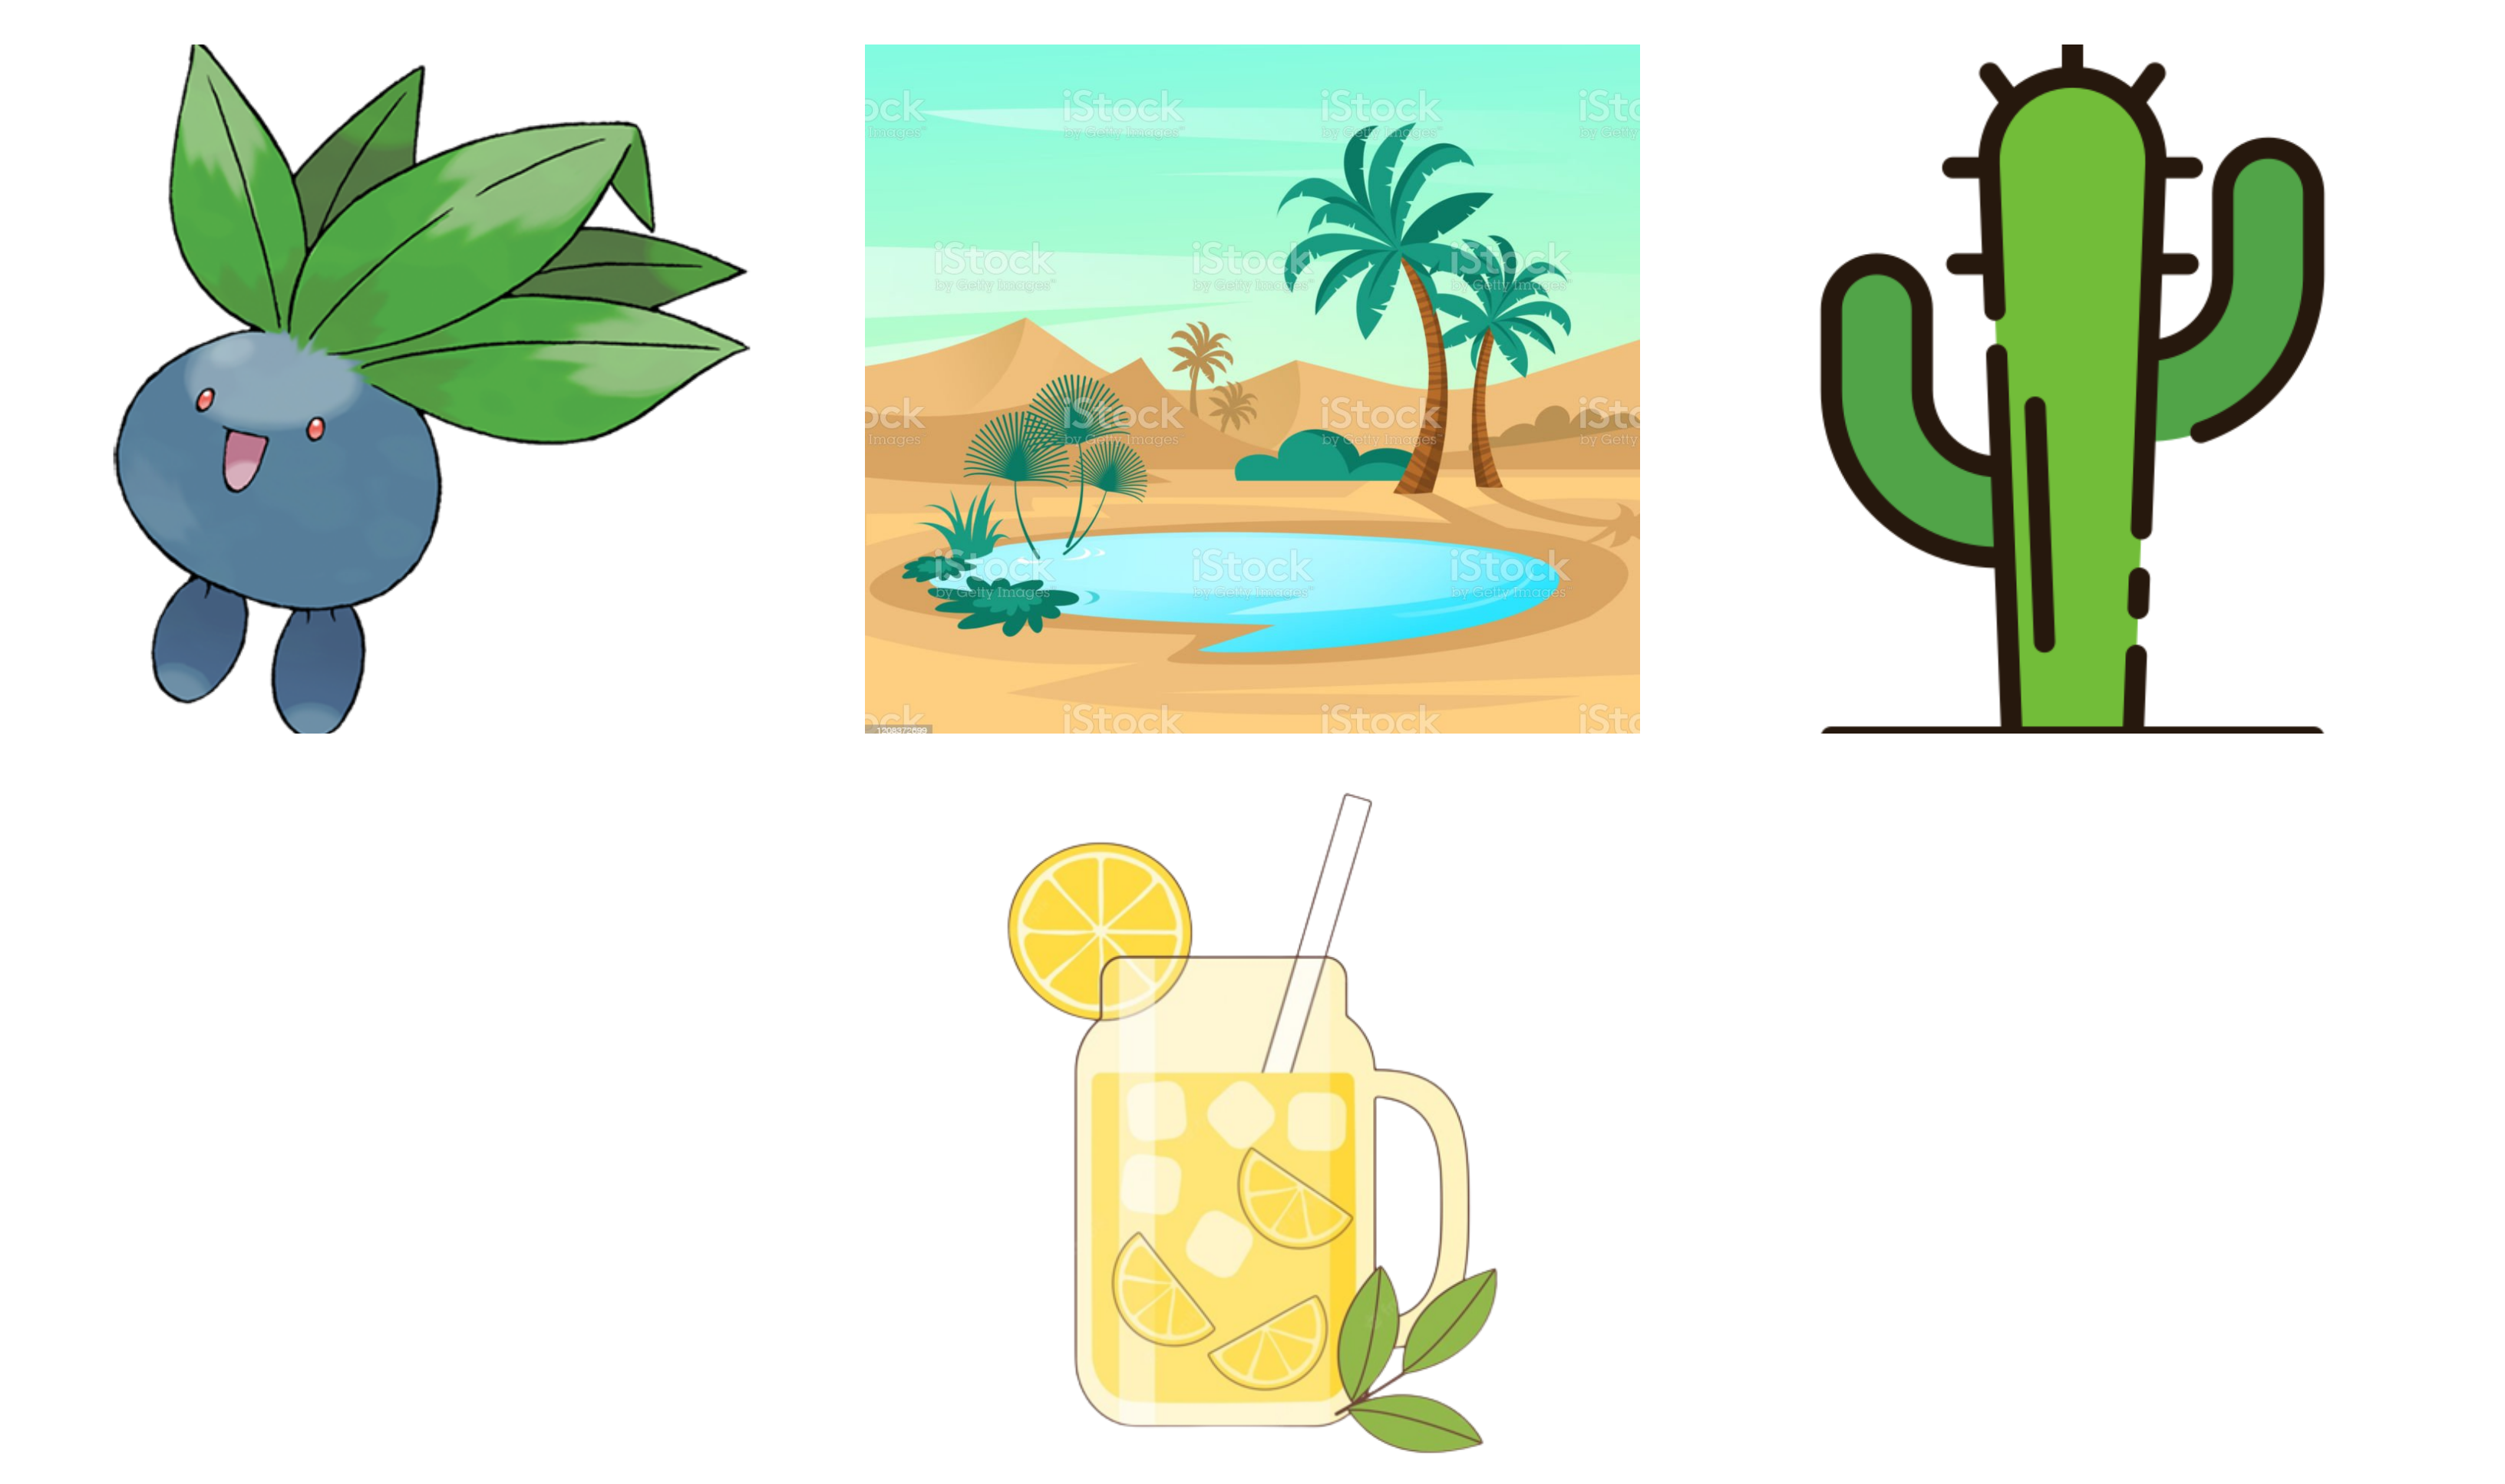
\includegraphics[width=\textwidth]{elements.png}
    \end{center}
    \caption{Environmental elements (from left to right; top to bottom) Agent, Goal,
        Negative Reward, Reward}
    \label{fig:elements}
\end{figure}

The enivironment is a \verb|6x6| grid defined according to the Gym \cite{1606.01540} API.
With \verb|36| possible positions that the agent can
occupy. The goal is to reach the oasis (shown in Figure \ref{fig:elements}) \textbf{after
consuming all} the juice (positive reward) within a (configurable) maximum number of time
steps. If the agent lands on a juice tile it is awarded +0.99 and the cactus (negative
reward) leads to a -1.0 reward. Once all the juice is consumed, the agent must proceed to the
oasis to earn a reward of +1.0
The states in this enviroment are a \textbf{combination} of the agent's position and the
currently available rewards (positive, negative and goal) on the grid. The Formula
\ref{eqn:num-states} gives us the number of possible states for the agent.

\begin{equation}
    num_{states}=num_{pos} \sum_{k=0}^{c_{reward}} {c_{reward}\choose k}
    \label{eqn:num-states}
\end{equation}

Here $num_{pos}$ refers to the number of grid squares, \verb|36| in our case. $c_{reward}$
refers to the number of positive rewards + the number of negative rewards + 1 (for the goal
state). We have \verb|6| negative rewards, \verb|3| positive rewards and one goal. Hence, 
the $num_{states}$ for us is \verb|36864|.

In each position our agent can take 4 potential actions:
\begin{enumerate*}
    \item Left
    \item Right
    \item Up
    \item Down.
\end{enumerate*}
Resetting the environment will not change the location or distribution of the rewards and
goal state. It only alters the initial state of the agent.

\begin{figure}[h]
    \begin{center}
        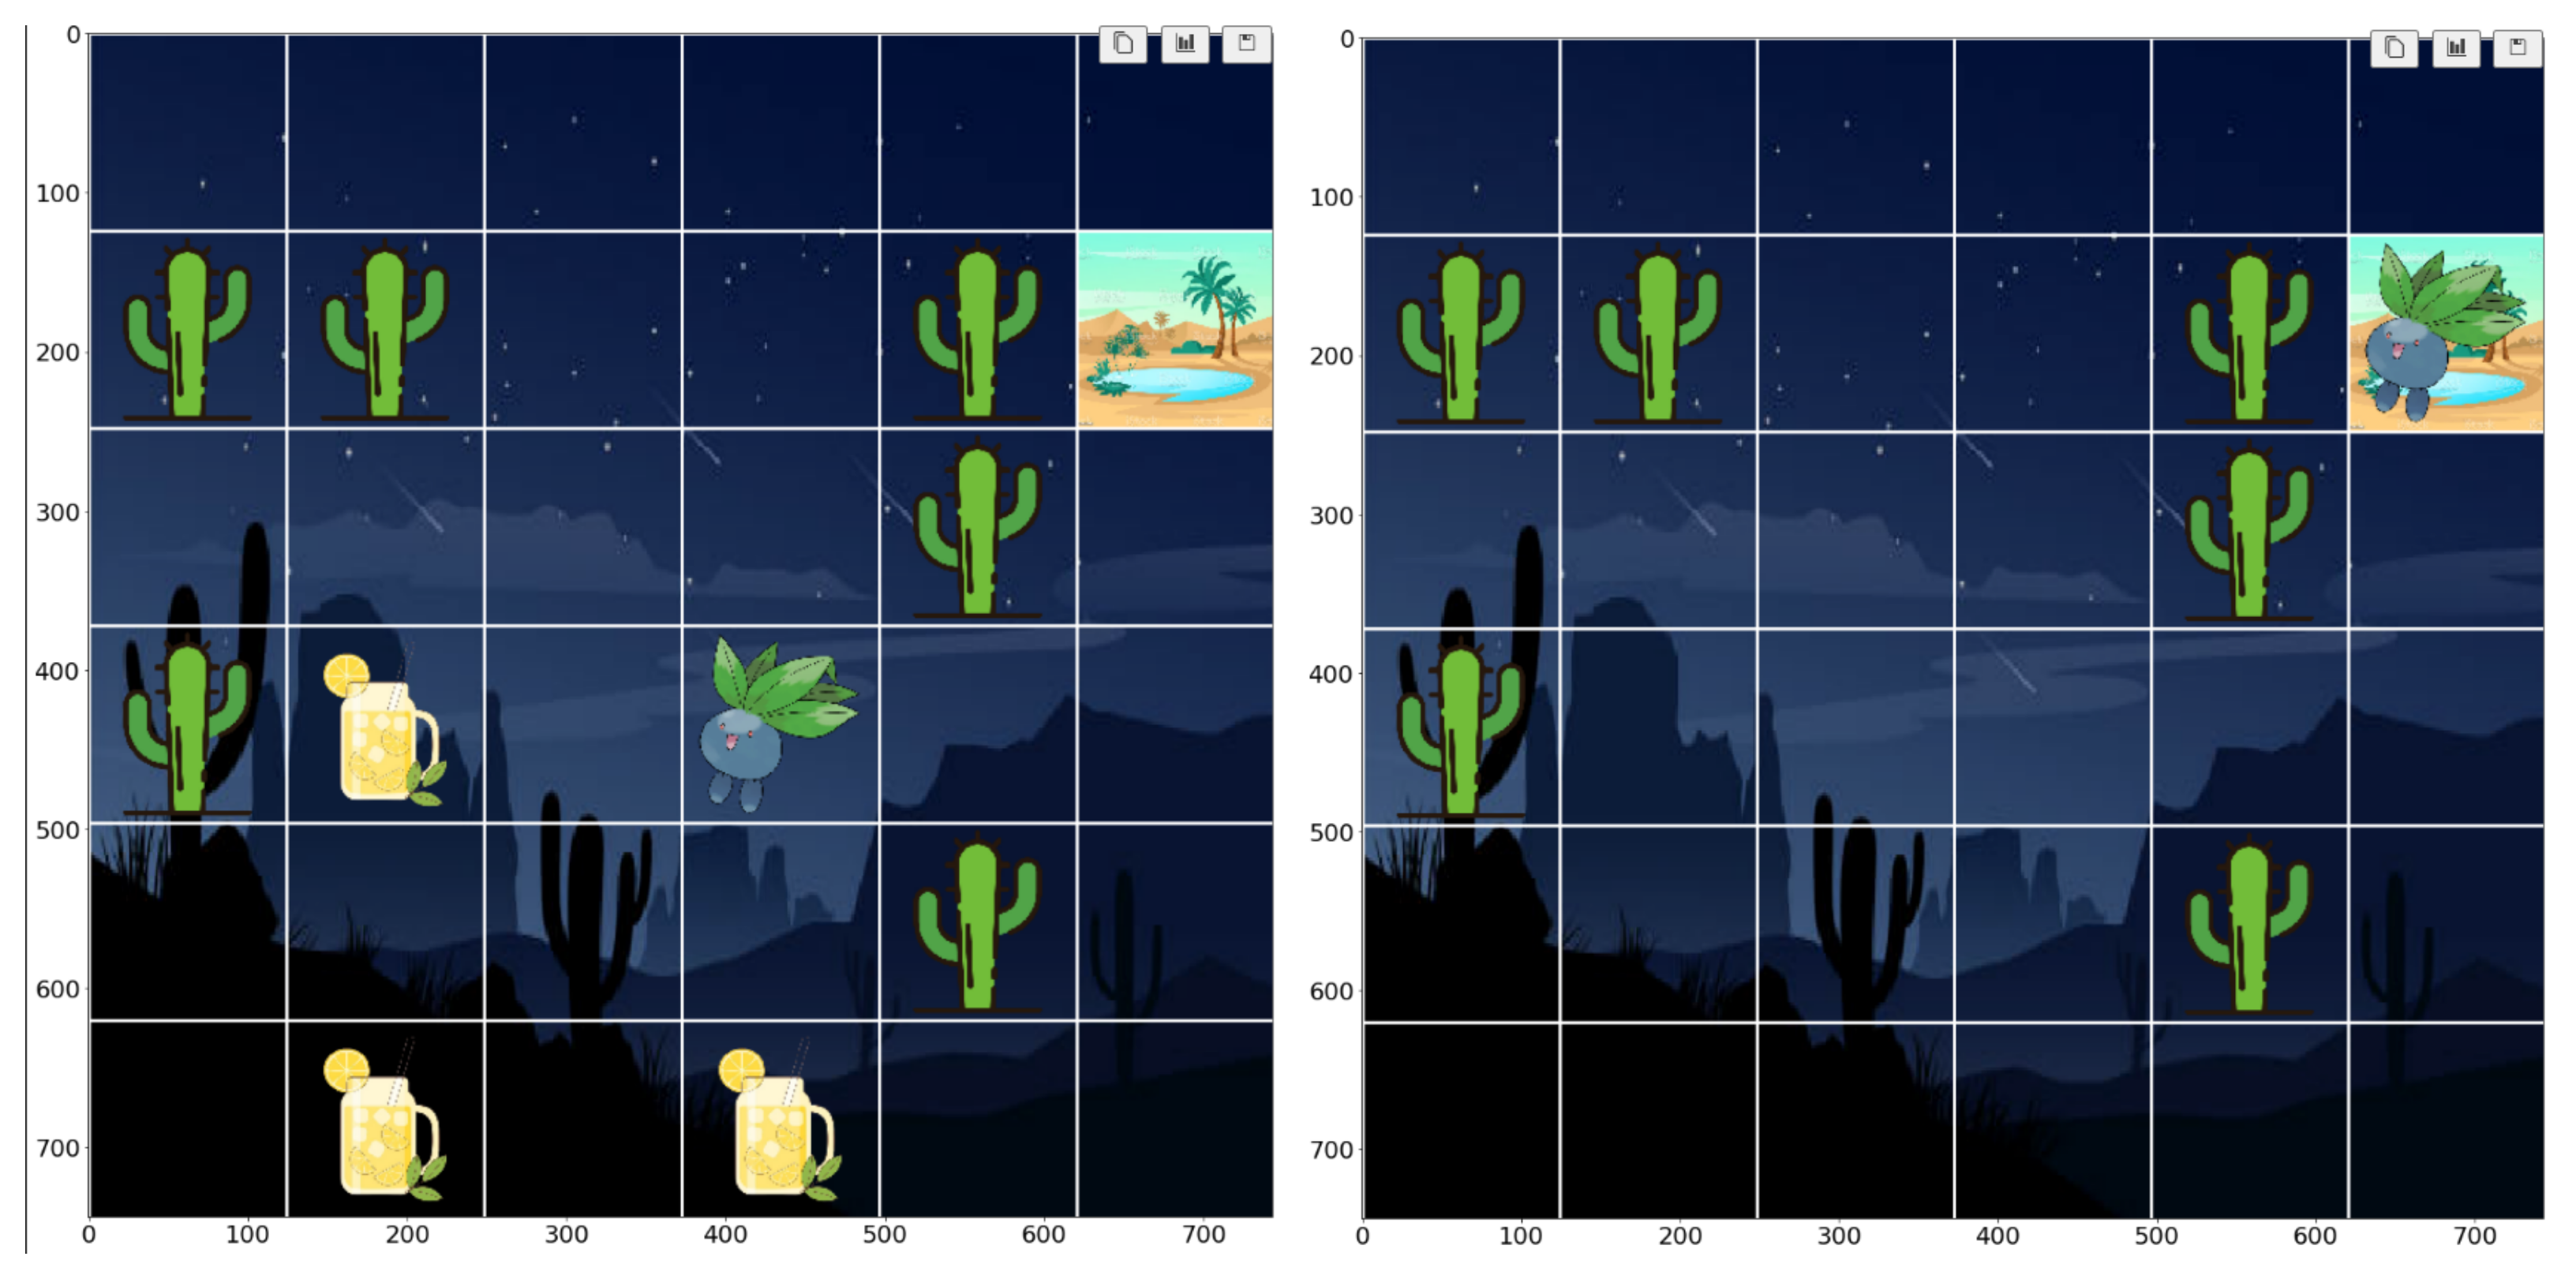
\includegraphics[scale=0.50]{vis.png}
    \end{center}
    \caption{Environment visualizations}
\end{figure}

\subsection{Safety in AI}
\label{sec:safety}
The following are properties of the environment that ensure valid behavior from the agent:

\begin{enumerate}
    \item We ensure that the agent consumes \textit{all} the \verb|pos_reward| and reaches
        the \verb|goal_state| in the fewest number of steps by imposing a penalty of \verb|0.1x|
        the \verb|max_reward| for every move made.
    \item The reward on all squares is consumed once the agent lands in that state, preventing 
    the agent from settling down in a \textit{high-reward} neighborhood.
    \item The result of any action (left, right, top, down) are clipped to the min and max
        values of 0 and \verb|GridSize| (6 in our case) respectively, ensuring that the
        agent never leaves the environment.
    \item If the agent makes a move but remains in the same spot, we impose the \textit{maximum negative
        reward} (-1.0 in our case). This allows the agent to disincentivize making fruitless
        moves.
    \item We also prevent a \textit{goal rush} (before the agent consumes all the positive
        rewards) by making the goal square unreachable when there are positive reward squares
        left. If the agent takes an action to move into a goal square before collecing all the
        \textit{positive rewards}, they will be kept on the same square, incurring an additional
        penalty (-1.0 in our case) as detailed in the previous point.
    \item The stocasticity of the starting point and limited time steps will nudge the agent
        to build strategies that accumulate the maximal reward in the shortest time.
\end{enumerate}

\section{CartPole-v1}
\label{sec:cart-definition}

In the cart-pole problem version described by Barto, Sutton, and Anderson 
\cite{barto1983neuronlike} a pole is
connected to a cart through a joint that cannot be moved. The cart can move on a track
without any friction. The pole is positioned upright on the cart and the objective is to
keep the pole balanced by applying forces to the cart in either the left or right direction.
This environment has been visualized in Figure \ref{fig:cartpole-rendering}.

\begin{figure}[h]
    \begin{center}
        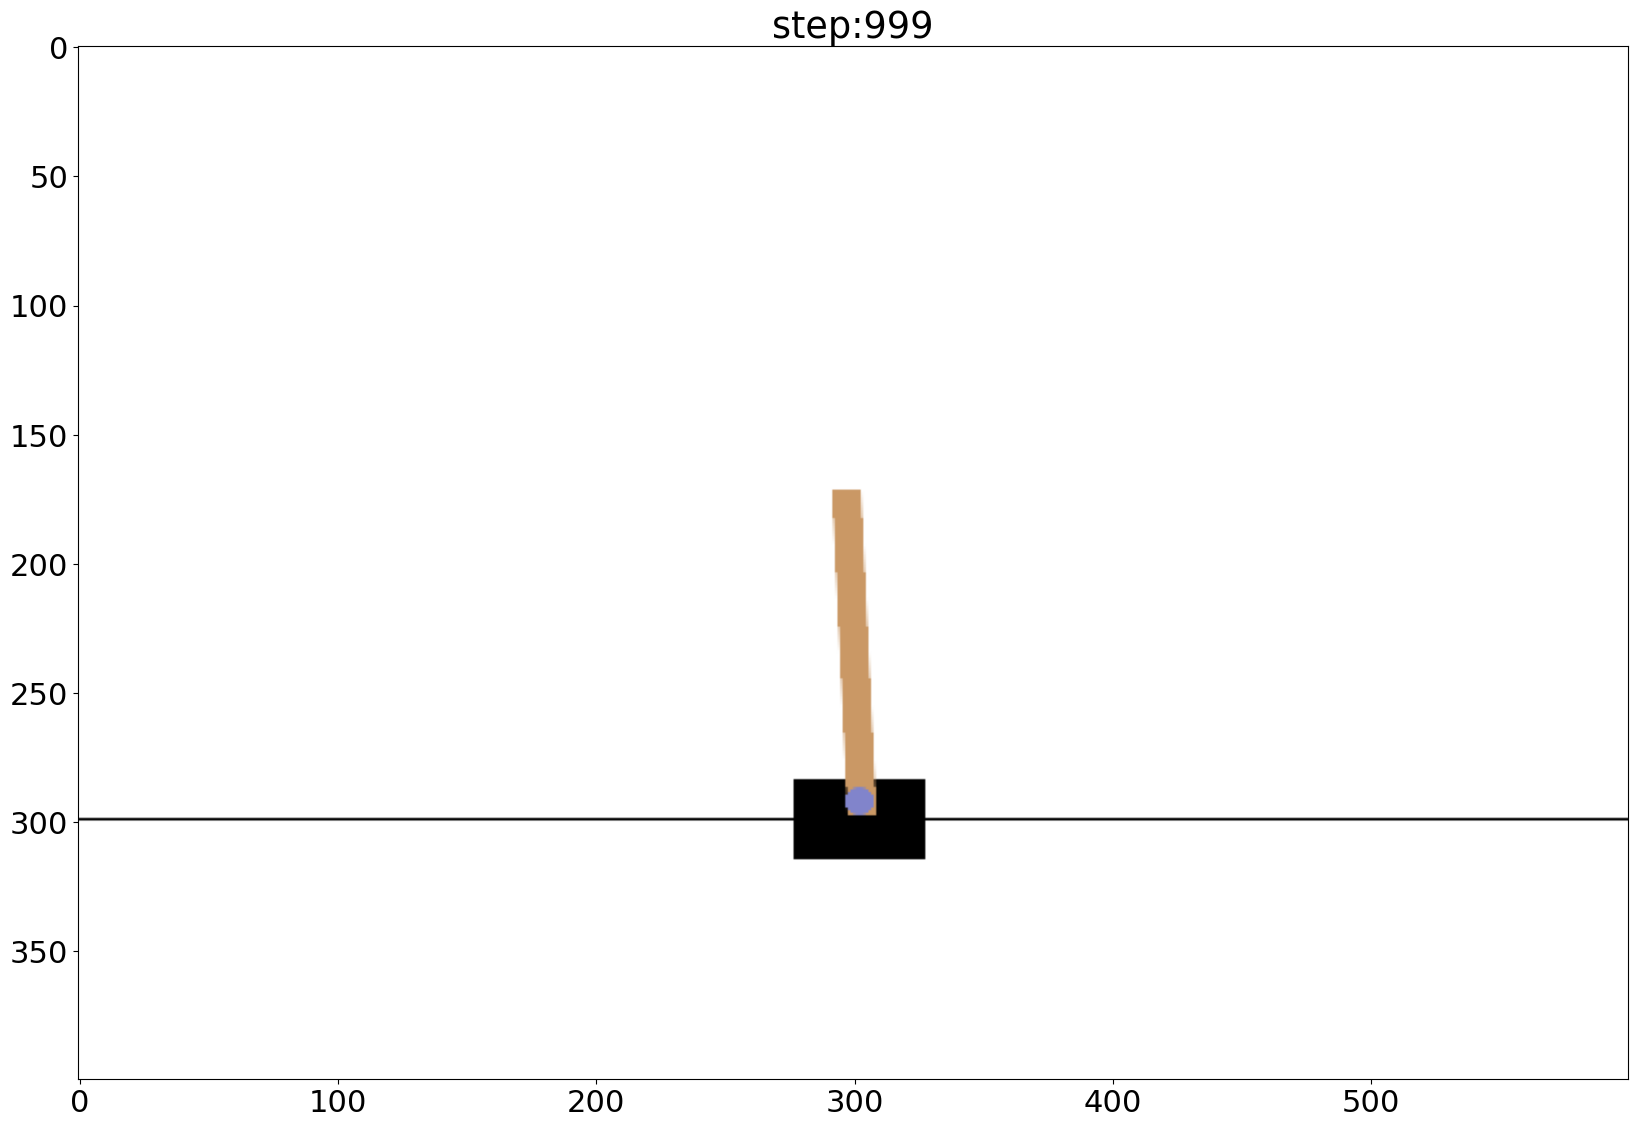
\includegraphics[width=\textwidth]{cartpole.png}
    \end{center}
    \caption{A frame from CartPole-v1}
    \label{fig:cartpole-rendering}
\end{figure}

\subsection{Action Space}
The action is an ndarray of shape (1,) that can take on values {0, 1} to indicate the
direction in which the cart is pushed with a fixed force.

\begin{itemize}
    \item 0: The cart is pushed to the left
    \item 1: The cart is pushed to the right
\end{itemize}

The velocity that is either decreased or increased by the force applied is not constant
and depends on the angle at which the pole is pointing. The center of gravity of the pole
affects the amount of energy required to move the cart beneath it.

\subsection{Observation Space}

The observation is an ndarray of shape (4,) where the values represent the positions and
velocities described next.

\begin{center}
    \begin{tabular}{cccc}
        \toprule
        Num & Observation & Min & Max \\
        \midrule
        0 & Cart Position & -4.8 & 4.8 \\
        1 & Cart Velocity & -Inf & Inf \\
        2 & Pole Angle & $\sim$ -0.418 rad (-24°) & $\sim$ 0.418 rad (24°) \\
        3 & Pole Angular Velocity & -Inf & Inf \\
        \bottomrule
    \end{tabular}
\end{center}

Although the ranges above indicate the possible values for each element in the observation
space, they do not reflect the allowed values of the state space in an ongoing episode.
Specifically:

\begin{itemize}
    \item The cart x-position (index 0) can be take values between \verb|(-4.8, 4.8)|,
    but the episode terminates if the cart leaves the \verb|(-2.4, 2.4)| range.
    \item The pole angle can be observed between \verb|(-.418, .418)| radians
    or \verb|(±24°)|, but the
    episode terminates if the pole angle is not in the range \verb|(-.2095, .2095)|
    or \verb|(±12°)|
\end{itemize}

\subsection{Rewards}

The objective of the task is to keep the pole upright for as long as possible. To encourage
this behavior, a reward of +1 is given for every step taken, including the final step when
the episode terminates. In version 1 of the task, the threshold for achieving a successful
outcome is set at 475.

\subsection{Start State}
All observations are assigned a uniformly random value in \verb|(-0.05, 0.05)|

\subsection{Episode End}
The episode terminates under these conditions:

\begin{enumerate}
    \item Termination: Pole Angle is greater than \verb|±12°|
    \item Termination: Cart Position is greater than \verb|±2.4| (center of the cart
    reaches the edge of the display)
    \item Truncation: Episode length is greater than \verb|500|
\end{enumerate}


\section{LunarLander-v2}

This environment represents a classic problem of optimizing rocket trajectory. Based on Pontryagin’s maximum principle, the optimal approach is to either fire the engine at full throttle or turn it off completely. As a result, this environment has discrete actions: the engine is either on or off.

Two versions of the environment are available: discrete and continuous. In our work we have used the discrete version. The landing pad is always located at coordinates \verb|(0,0)|, which are represented by the first two numbers in the state vector. It is possible to land outside of the landing pad. Since fuel is unlimited, an agent can learn to fly and land successfully on its first attempt.

\begin{figure}[h]
    \begin{center}
        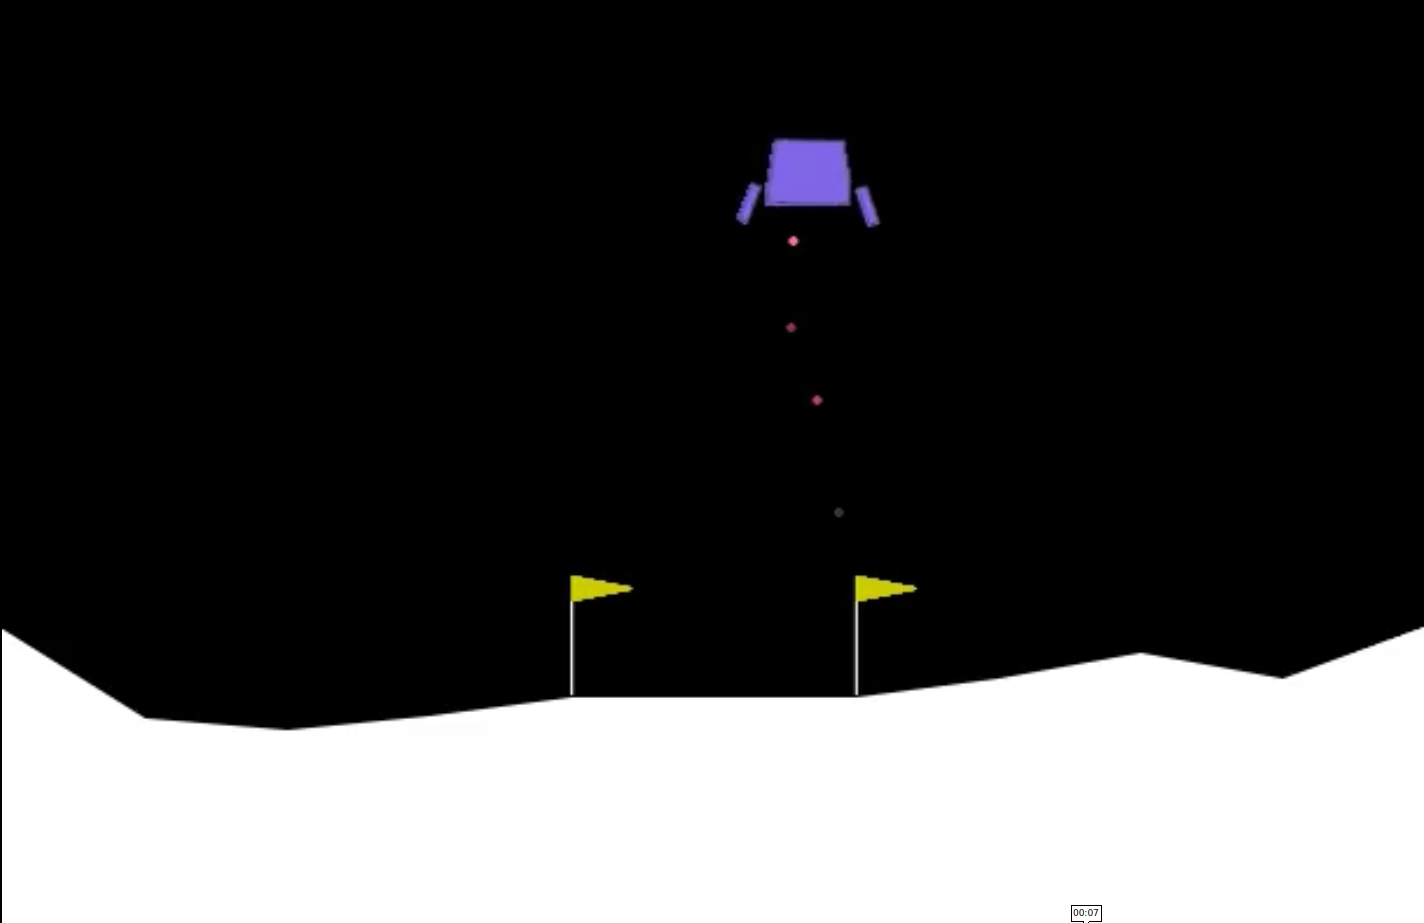
\includegraphics[width=\textwidth]{lunar_lander.png}
    \end{center}
    \caption{A frame from LunarLander-v2}
    \label{fig:mcar-rendering}
\end{figure}

\subsection{Observation Space}
The state of the environment is represented by an 8-dimensional vector that includes the \verb|x| and \verb|y| coordinates of the lander, its linear velocities in \verb|x| and \verb|y|, its angle and angular velocity, and two boolean values indicating whether each leg is in contact with the ground.

\subsection{Action Space}
Four discrete actions are available in this environment: remain idle, activate the left orientation engine, activate the main engine, or activate the right orientation engine.

\subsection{Reward}

A reward is given after each step in the environment. The total reward for an episode is calculated by summing the rewards for all steps within that episode. The reward for each step is determined by the following factors: \begin{itemize} \item The reward increases/decreases as the lander gets closer/further from the landing pad. \item The reward increases/decreases as the lander moves slower/faster. \item The reward decreases as the lander tilts more (angle not horizontal). \item The reward increases by 10 points for each leg in contact with the ground. \item The reward decreases by 0.03 points for each frame a side engine is firing. \item The reward decreases by 0.3 points for each frame the main engine is firing. \end{itemize} An additional reward of -100 or +100 points is given for crashing or landing safely, respectively. An episode is considered solved if it scores at least 200 points.

\subsection{Starting State}
At the beginning of each episode, the lander is positioned at the top center of the viewport and a random initial force is applied to its center of mass.


\subsection{Episode End}
An episode terminates if any of the following conditions are met: \begin{enumerate} \item The lander crashes (its body comes into contact with the moon). \item The lander moves outside of the viewport (its \verb|x| coordinate is greater than 1). \item The lander is not awake. According to the Box2D documentation, a body that is not awake does not move or collide with any other body. \end{enumerate}

\section{Discuss the benefits of:}
\subsection{Using experience replay in DQN and how its size can influence the results}

The experience replay in DQN helps to curb the problem of correlation between consecutive input samples to the training network which otherwise causes the network to diverge or make it unstable. The experience relay ensures the samples are i.i.d (independent and identically distributed) by randomizing them among batches by same distribution and are kept independent of each other in the same batch. This avoids the overfitting of some group of consecutive samples as the temporal variation is poor. 
The experience relay provides the opportunity to train the network by considering a large pool of samples already trained. There is a tradeoff between choosing the buffer size and the final outcome of such choice. Generally a small size buffer helps to learn the environment rapidly at the cost of ignoring the previous experiences. Similarly a larger buffer suffers from slow learning 

\subsection{Introducing the target network:}
The target network helps to avoid oscillation in policy as conventional Q value update changes the current estimate and target value. If the target Q value is impacted by the current update of the Q value, the training chases a non stationary target and does not help much in learning efficiently. WIth the introduction of a target network which is updated with the primary network only after some particular interval  helps to train the model effectively.

\subsection{Representing the Q function as \textit{q'(s, w)}}
This solves the problem of dealing with larger state-action domains or complex networks as the neural network representation can now serve  as  function approximation. The design matrix now reduces to updating the weight of the network to minimize the loss of the estimate and target network.

\section{Show and discuss your results after applying your DQN implementation on the three environments.}

\subsection{GridWorld}

We represent the current state of the environment as a 36 dimensional vector of rank 1. Here each
component of the vector has one of 3 values which indicate:

\begin{itemize}
    \item[$0.5$:] Agent location
    \item[$-1.0$:] Negative reward
    \item[$0.99$:] Positive reward
    \item[$1.0$:] Goal square
\end{itemize}

We feed this vector to a \verb|Feed-forward Network| that will give us the estimated
action-values. Then We take the \verb|argmax| over these action-values. We consider the
environments as solved when we have achieved a 100 episode running average of $~2.1$.

\subsection{CartPole-v1 \& LunarLander-v2}
For both these environments we have rather similar action spaces (\verb|Discrete|), hence the
\verb|Feed-forward Network| architechture used is also similar. The input of the network has the shape
\verb|1 x state-space| output of network will \verb|1 x action-space|.

The enivironments are considered solved when:
\begin{itemize}
    \item[] \textbf{CartPole-v1} Running average reward of 500 (100 episodes)
    \item[] \textbf{LunarLander-v2} Running average reward $>$ 200 (100 episodes)
\end{itemize}


\subsection{Training Discussion}

\begin{figure}[H]
    \begin{center}
        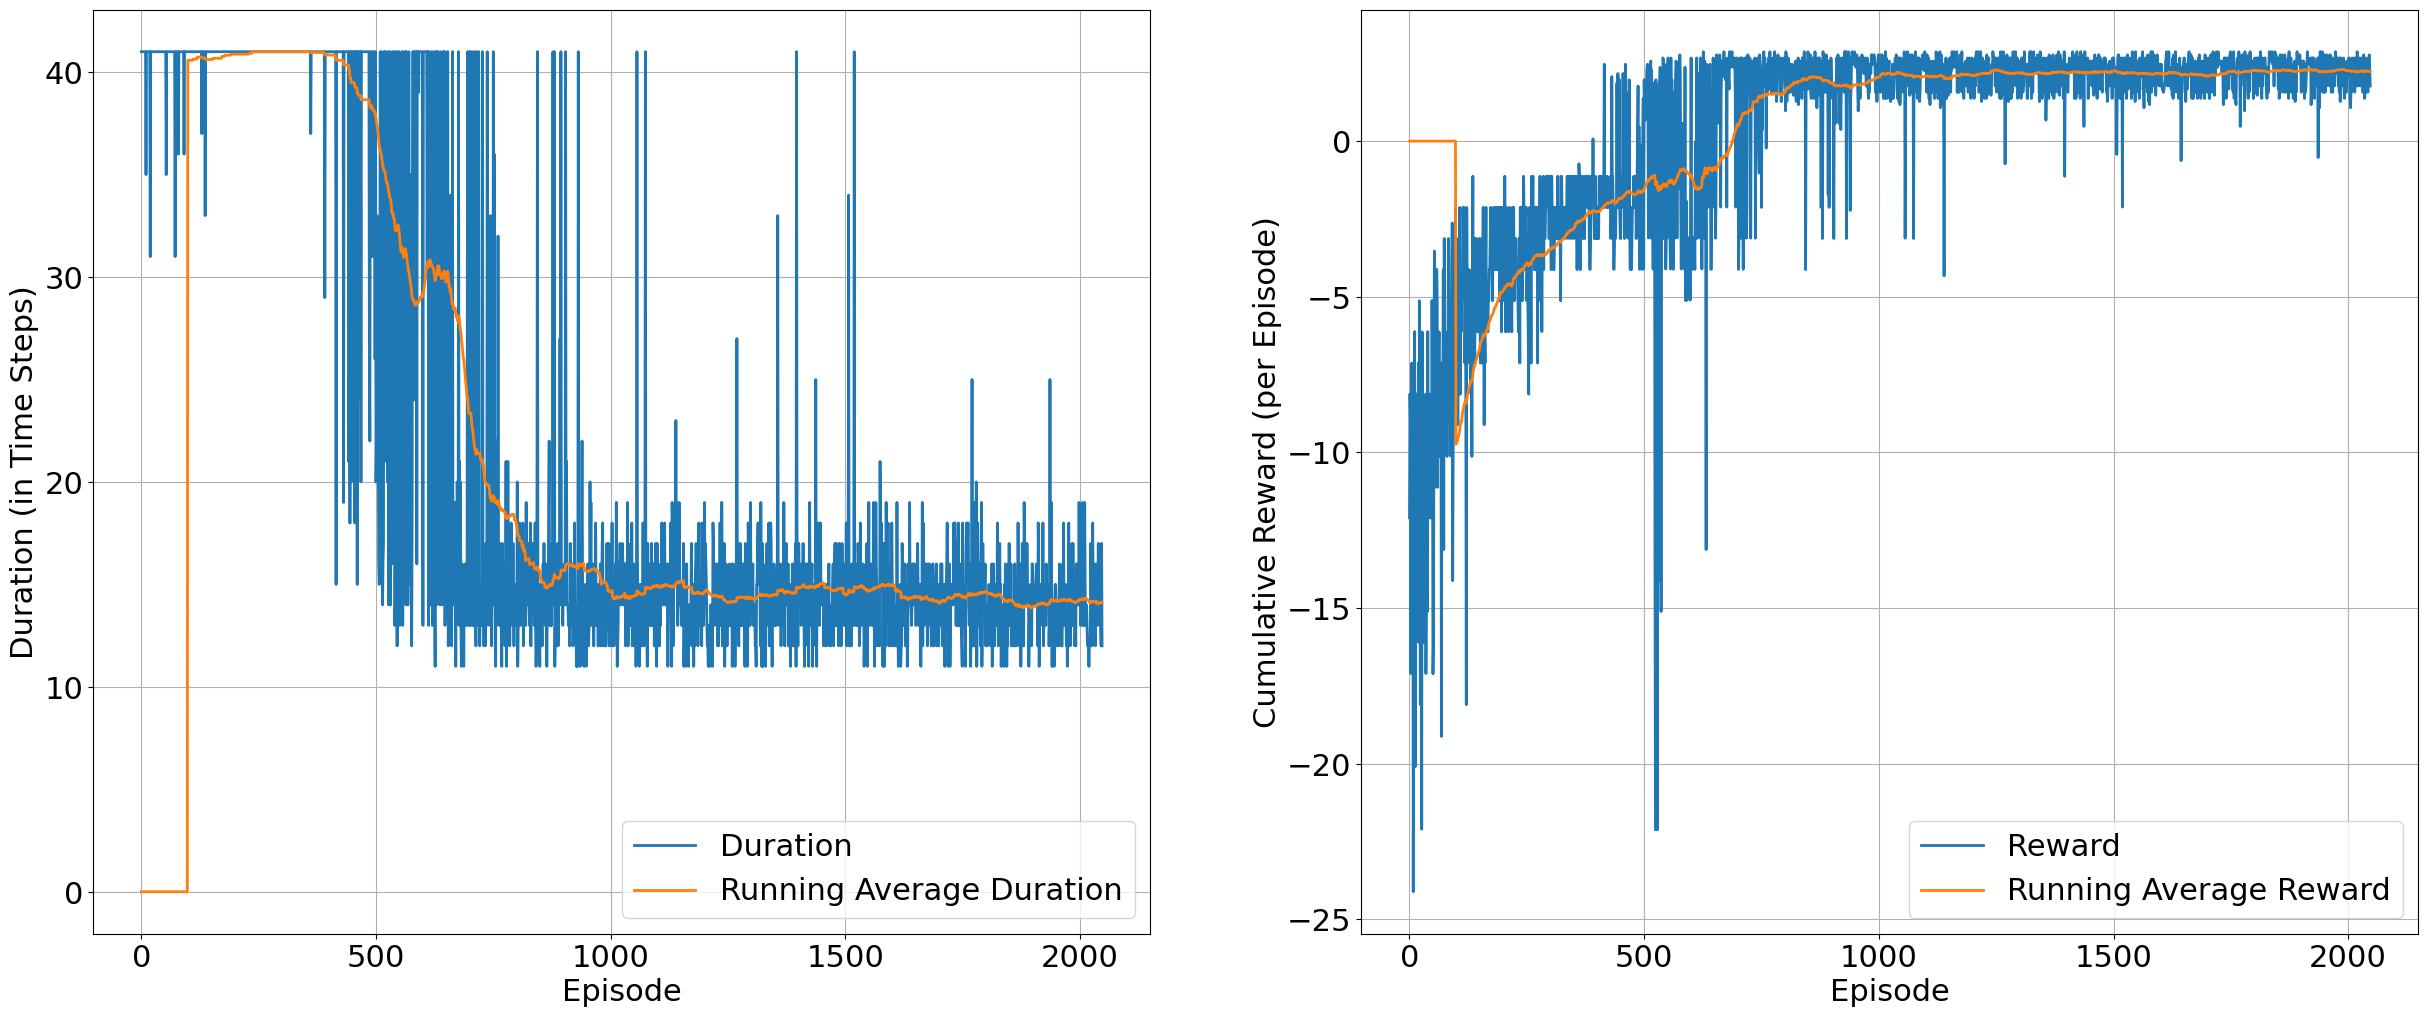
\includegraphics[width=\textwidth]{grid_training_ddqn.png}
    \end{center}
    \caption{Grid Training}
\end{figure}

\begin{figure}[H]
    \begin{center}
        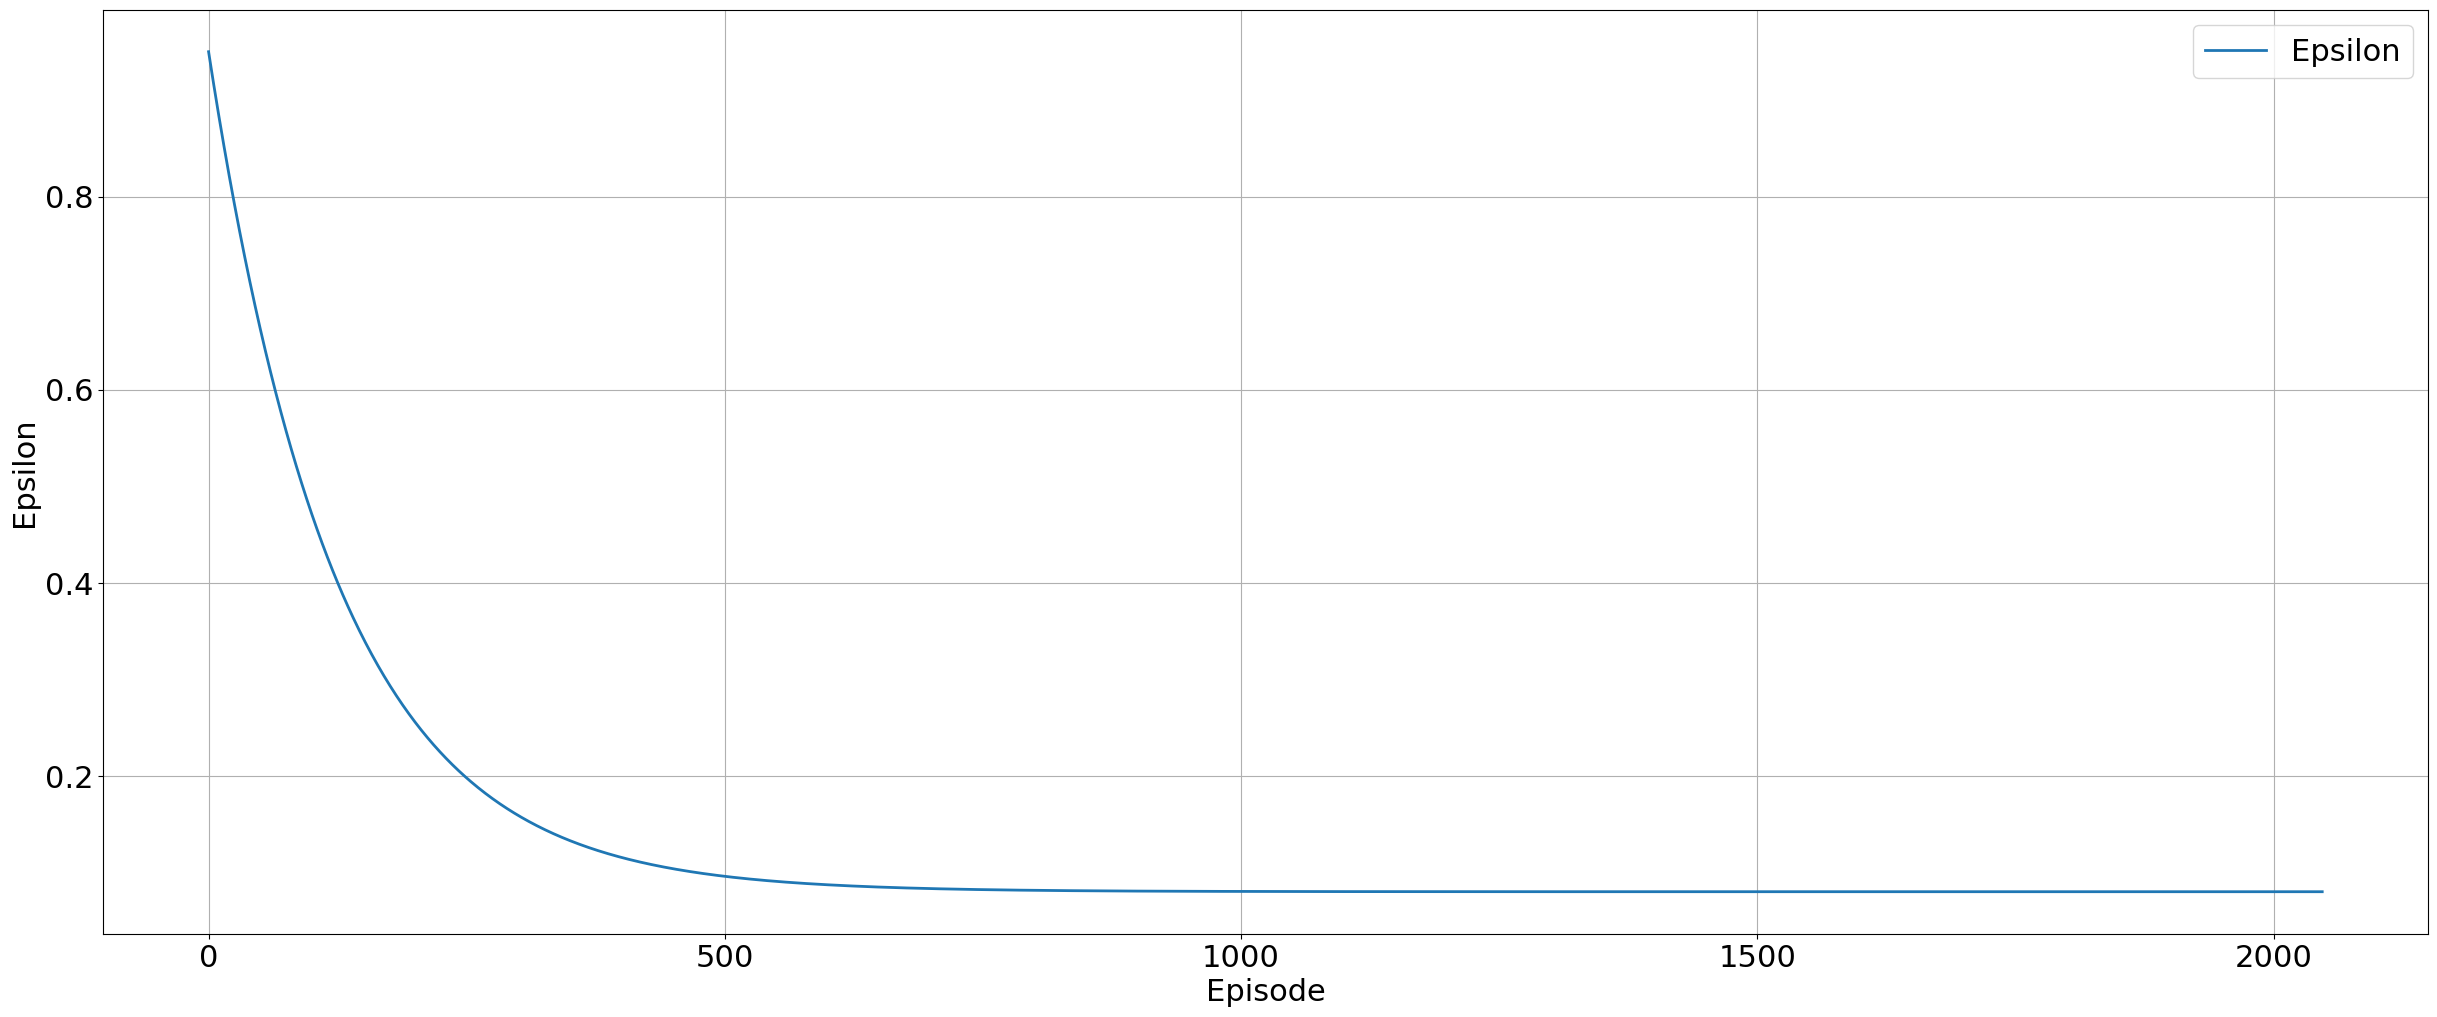
\includegraphics[width=\textwidth]{eps_grid_ddqn.png}
    \end{center}
    \caption{Epsilon Decay -- Grid Env}
\end{figure}

\begin{figure}[H]
    \begin{center}
        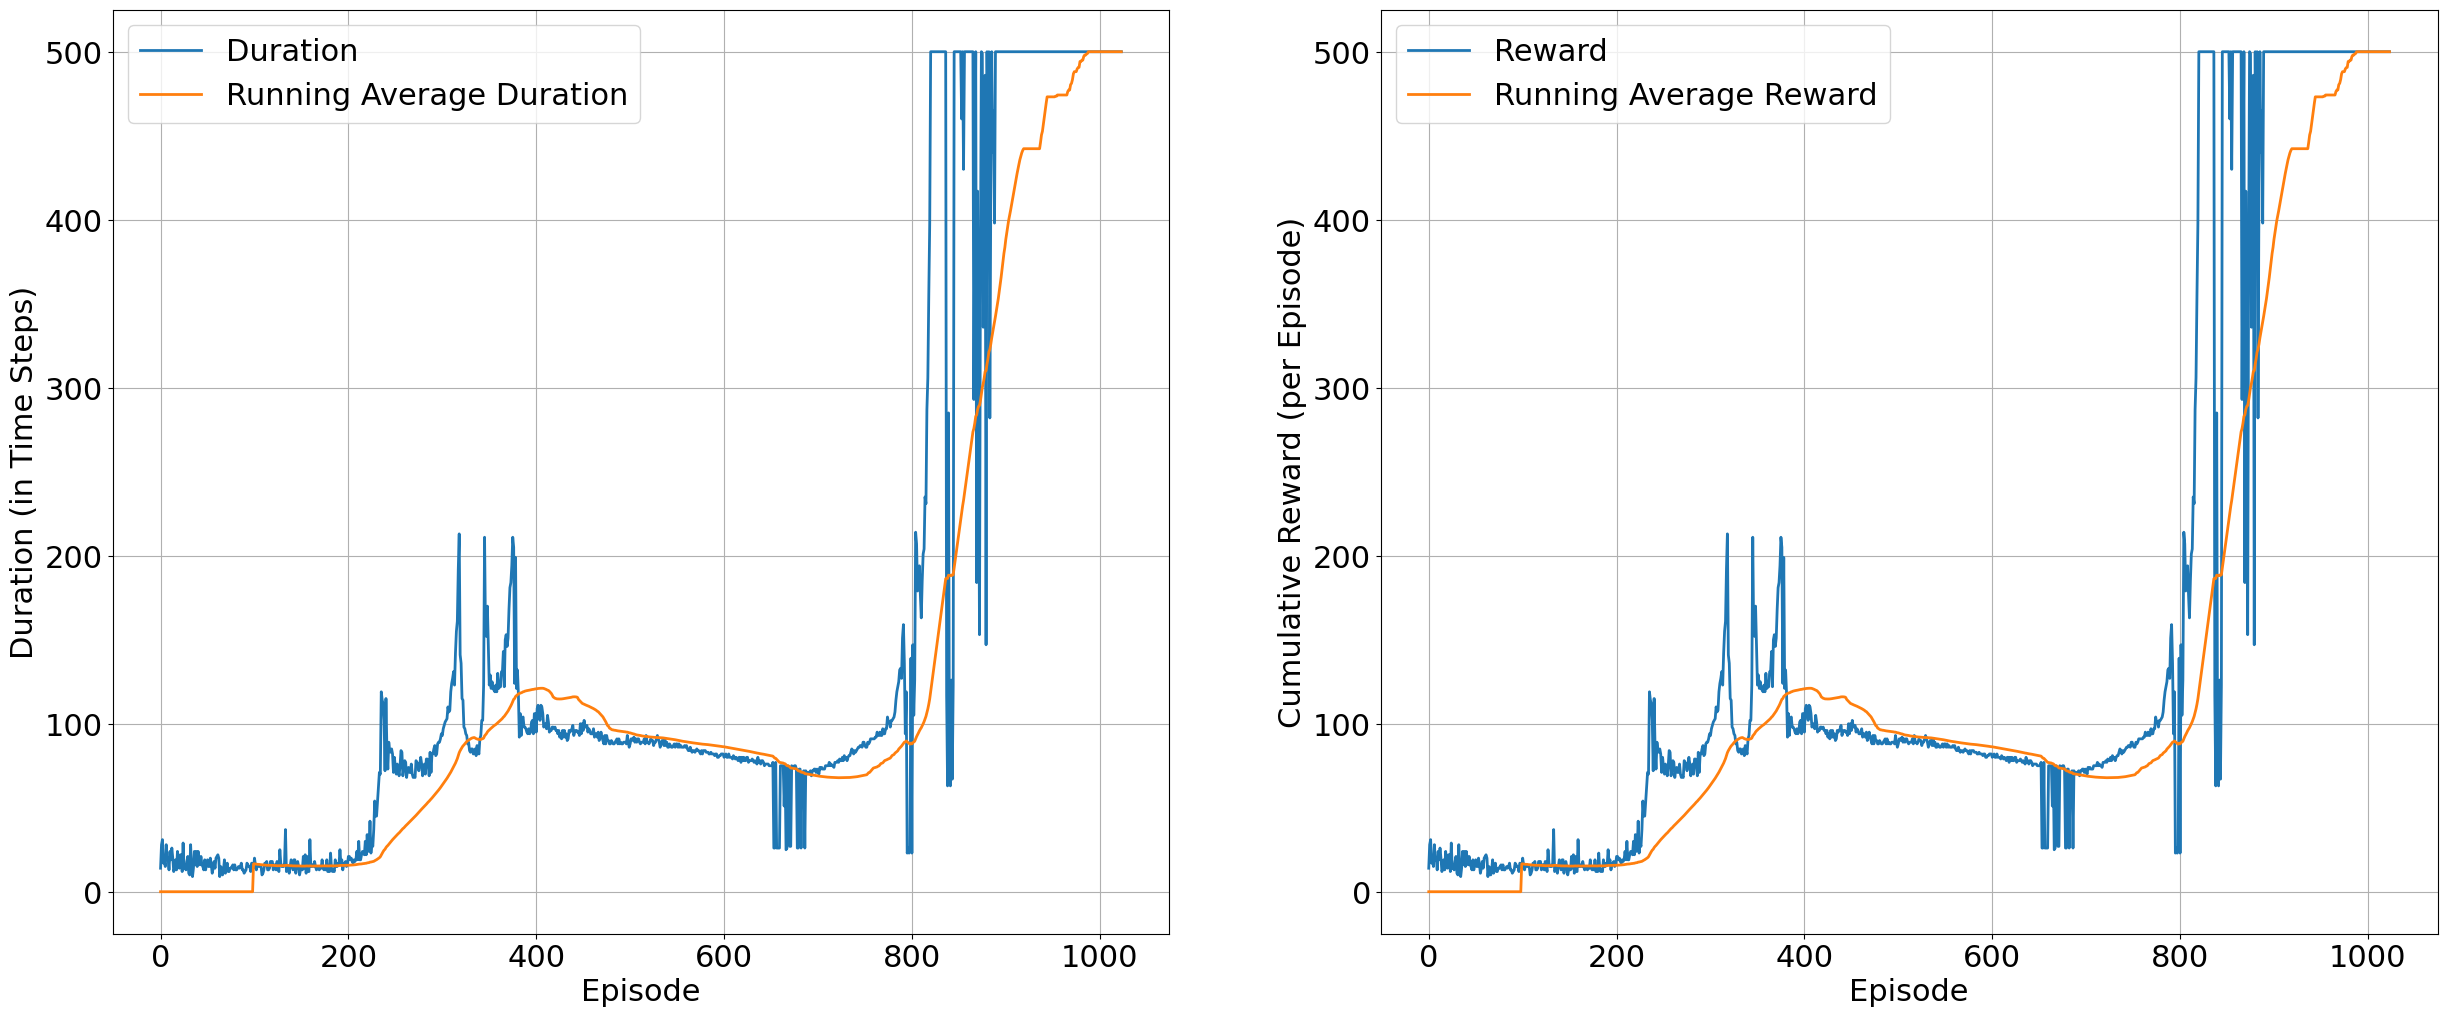
\includegraphics[width=\textwidth]{cartpole_training.png}
    \end{center}
    \caption{Cart-Pole Training}
\end{figure}

\begin{figure}[H]
    \begin{center}
        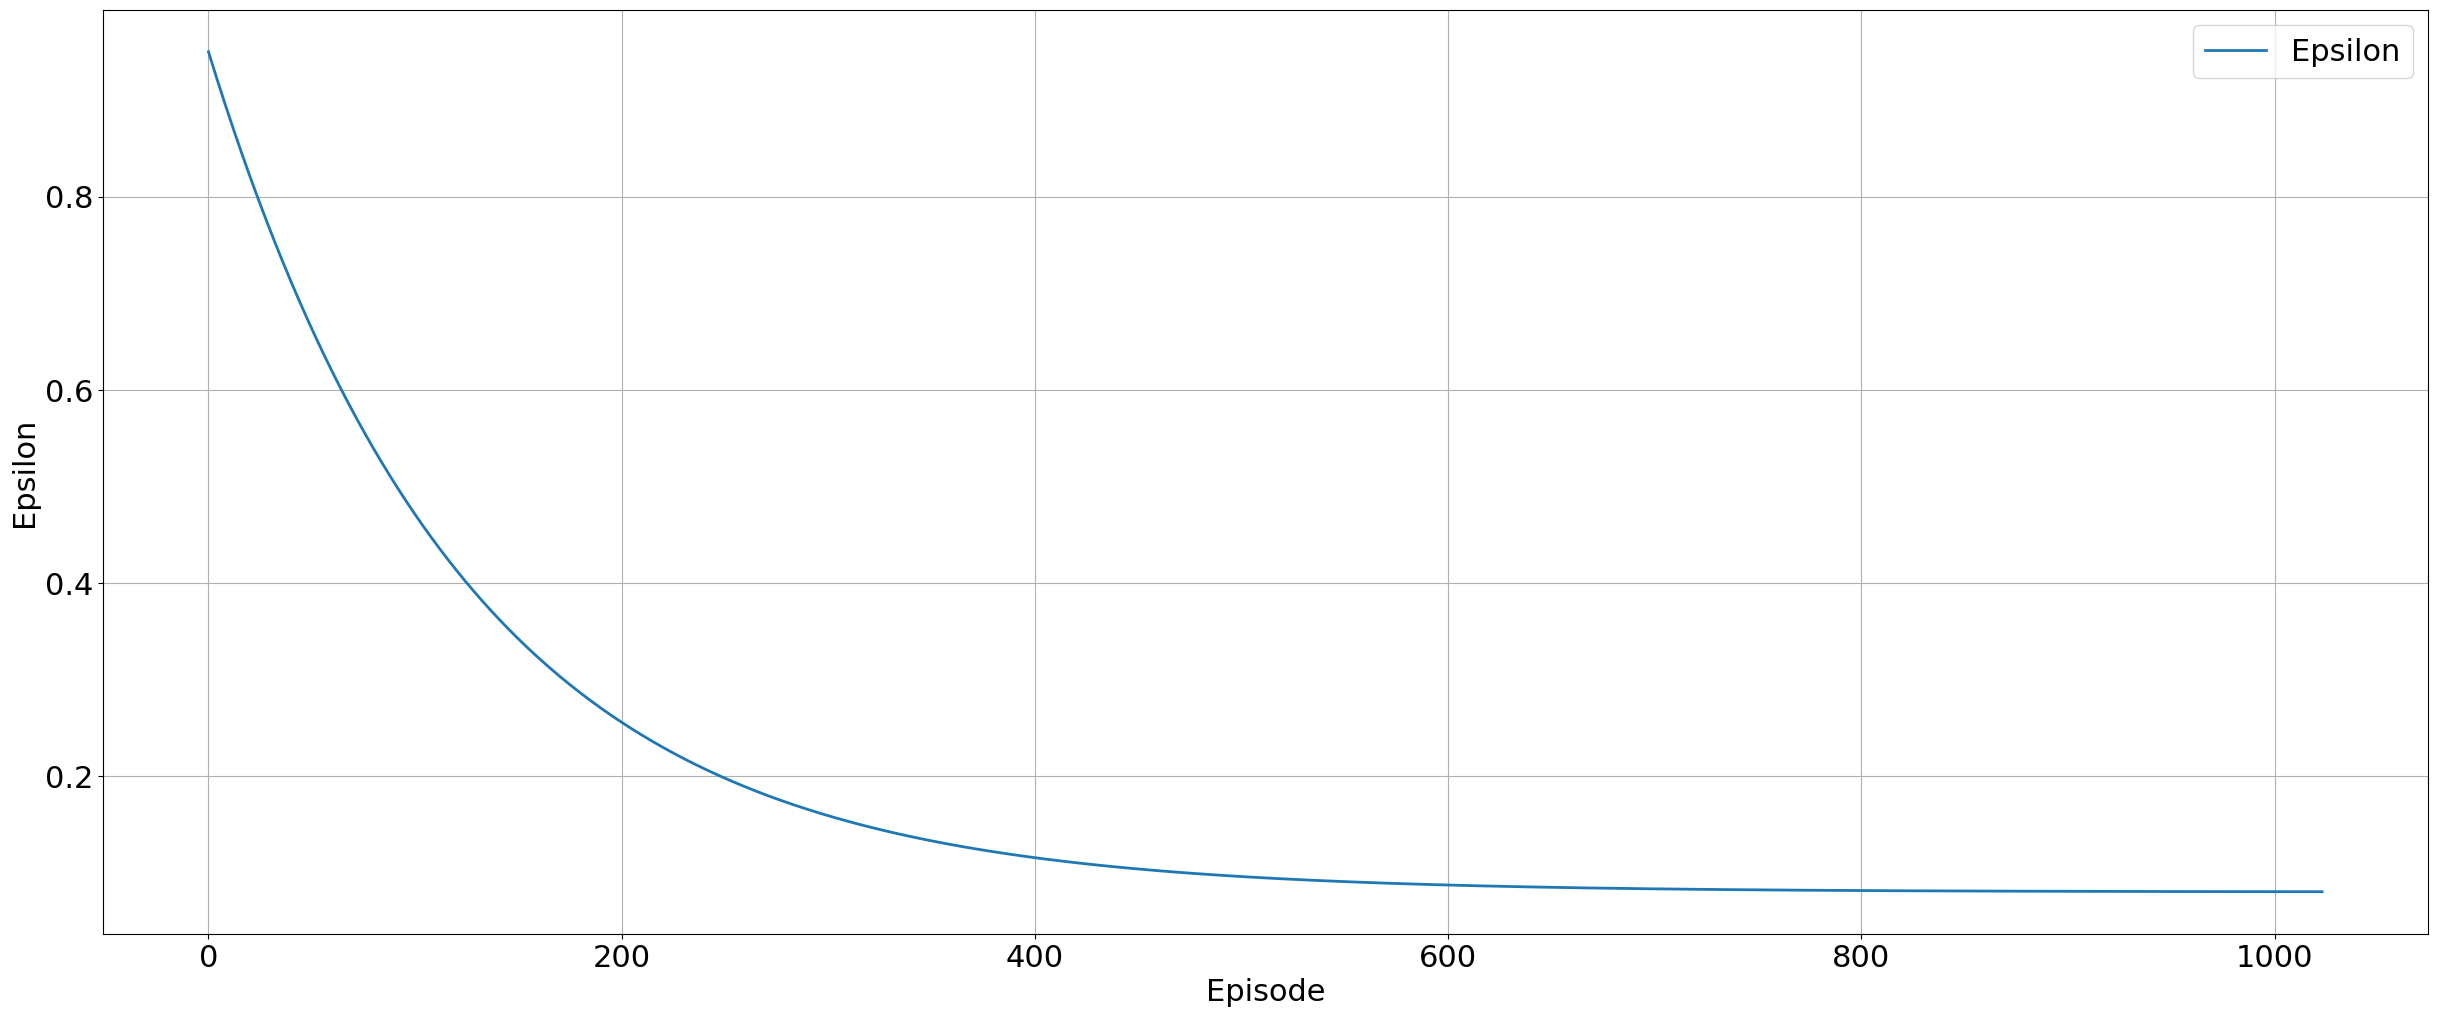
\includegraphics[width=\textwidth]{eps_cart.png}
    \end{center}
    \caption{Epsilon Decay -- Cart Pole}
\end{figure}

\begin{figure}[H]
    \begin{center}
        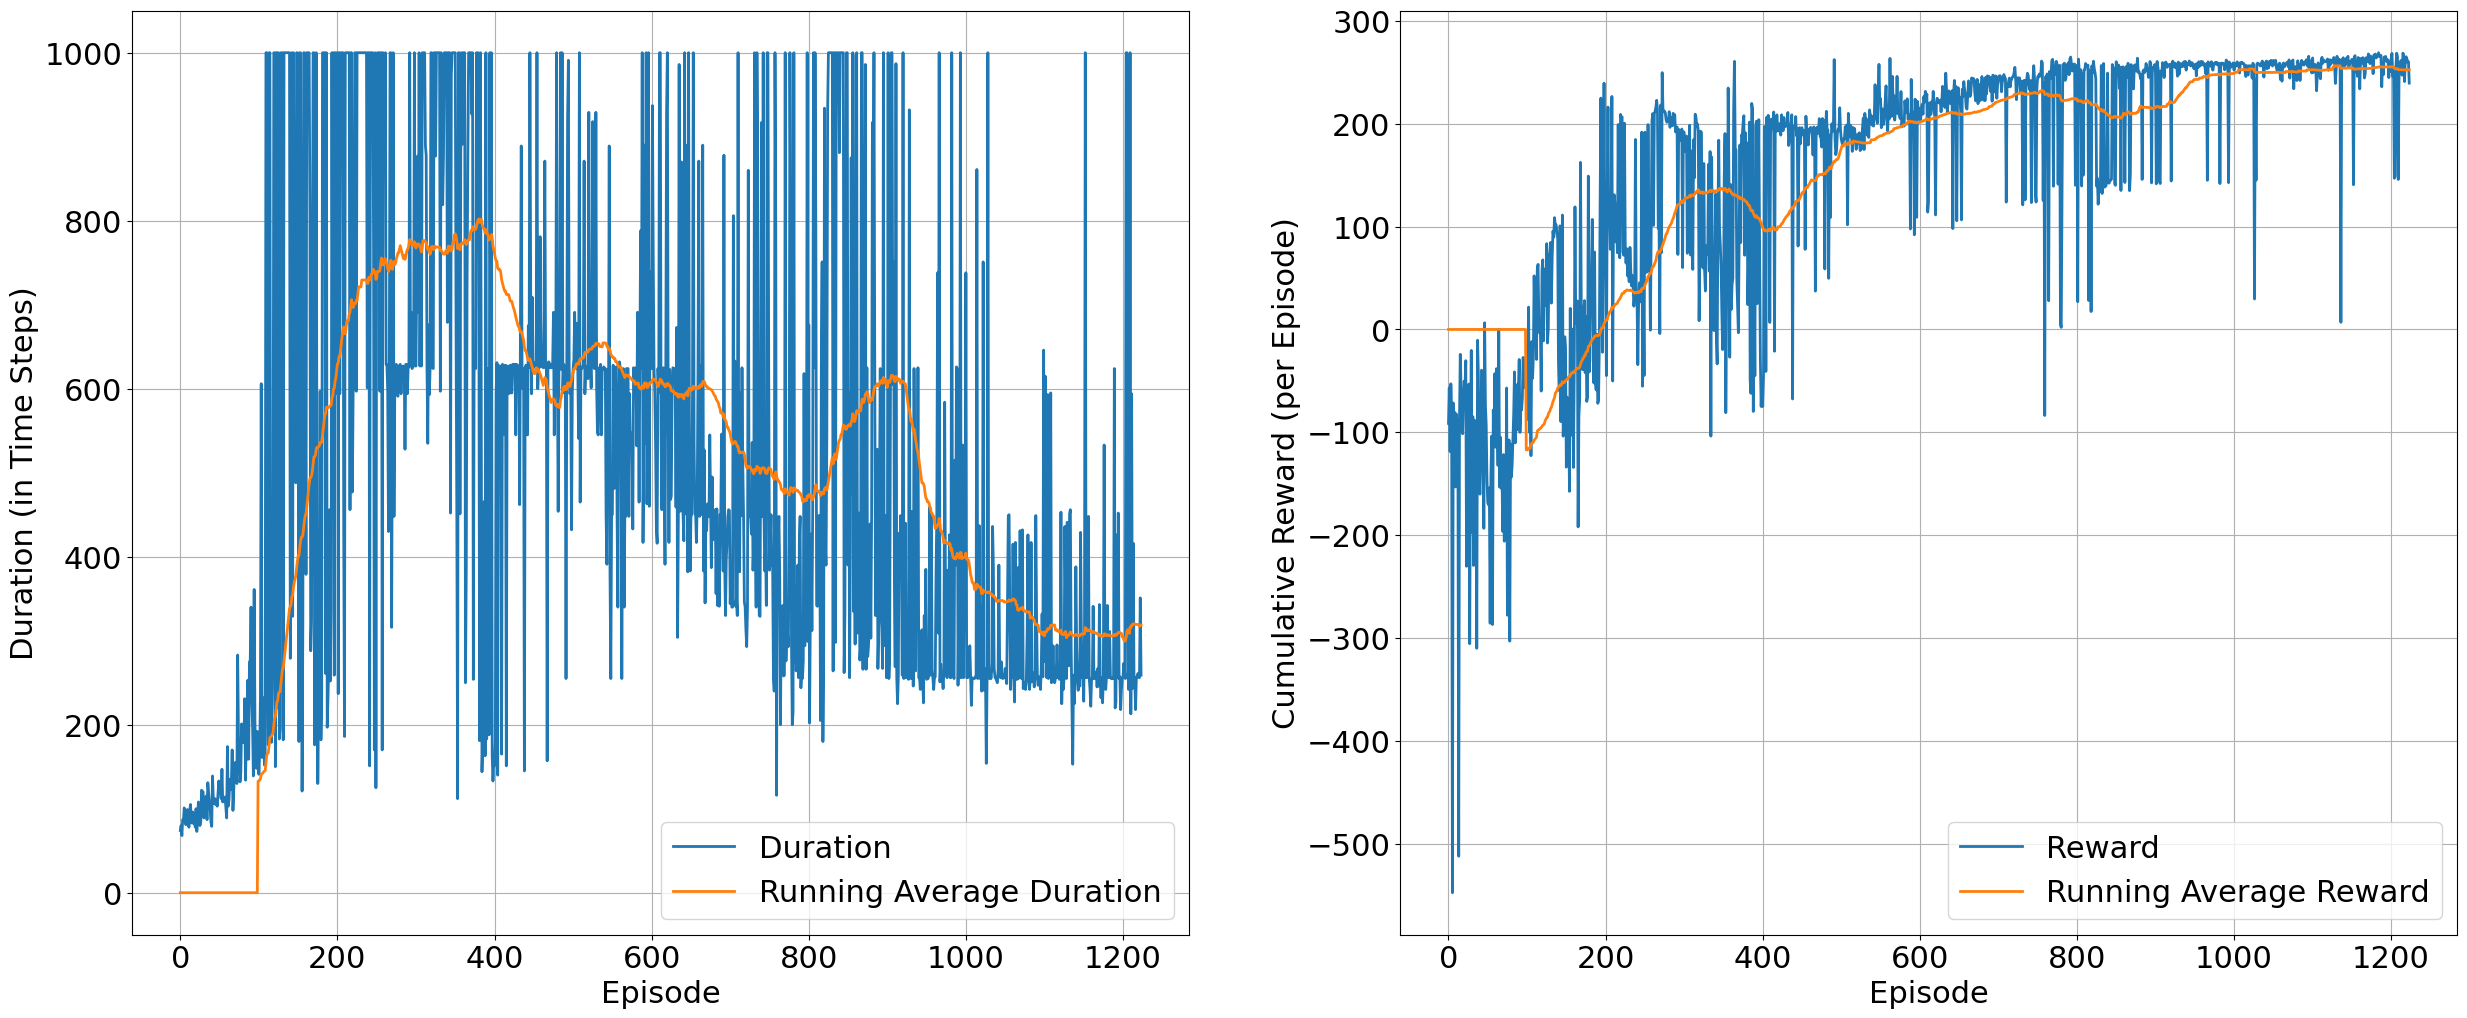
\includegraphics[width=\textwidth]{lunar_training_ddqn.png}
    \end{center}
    \caption{Lunar Lander Training}
\end{figure}

\begin{figure}[H]
    \begin{center}
        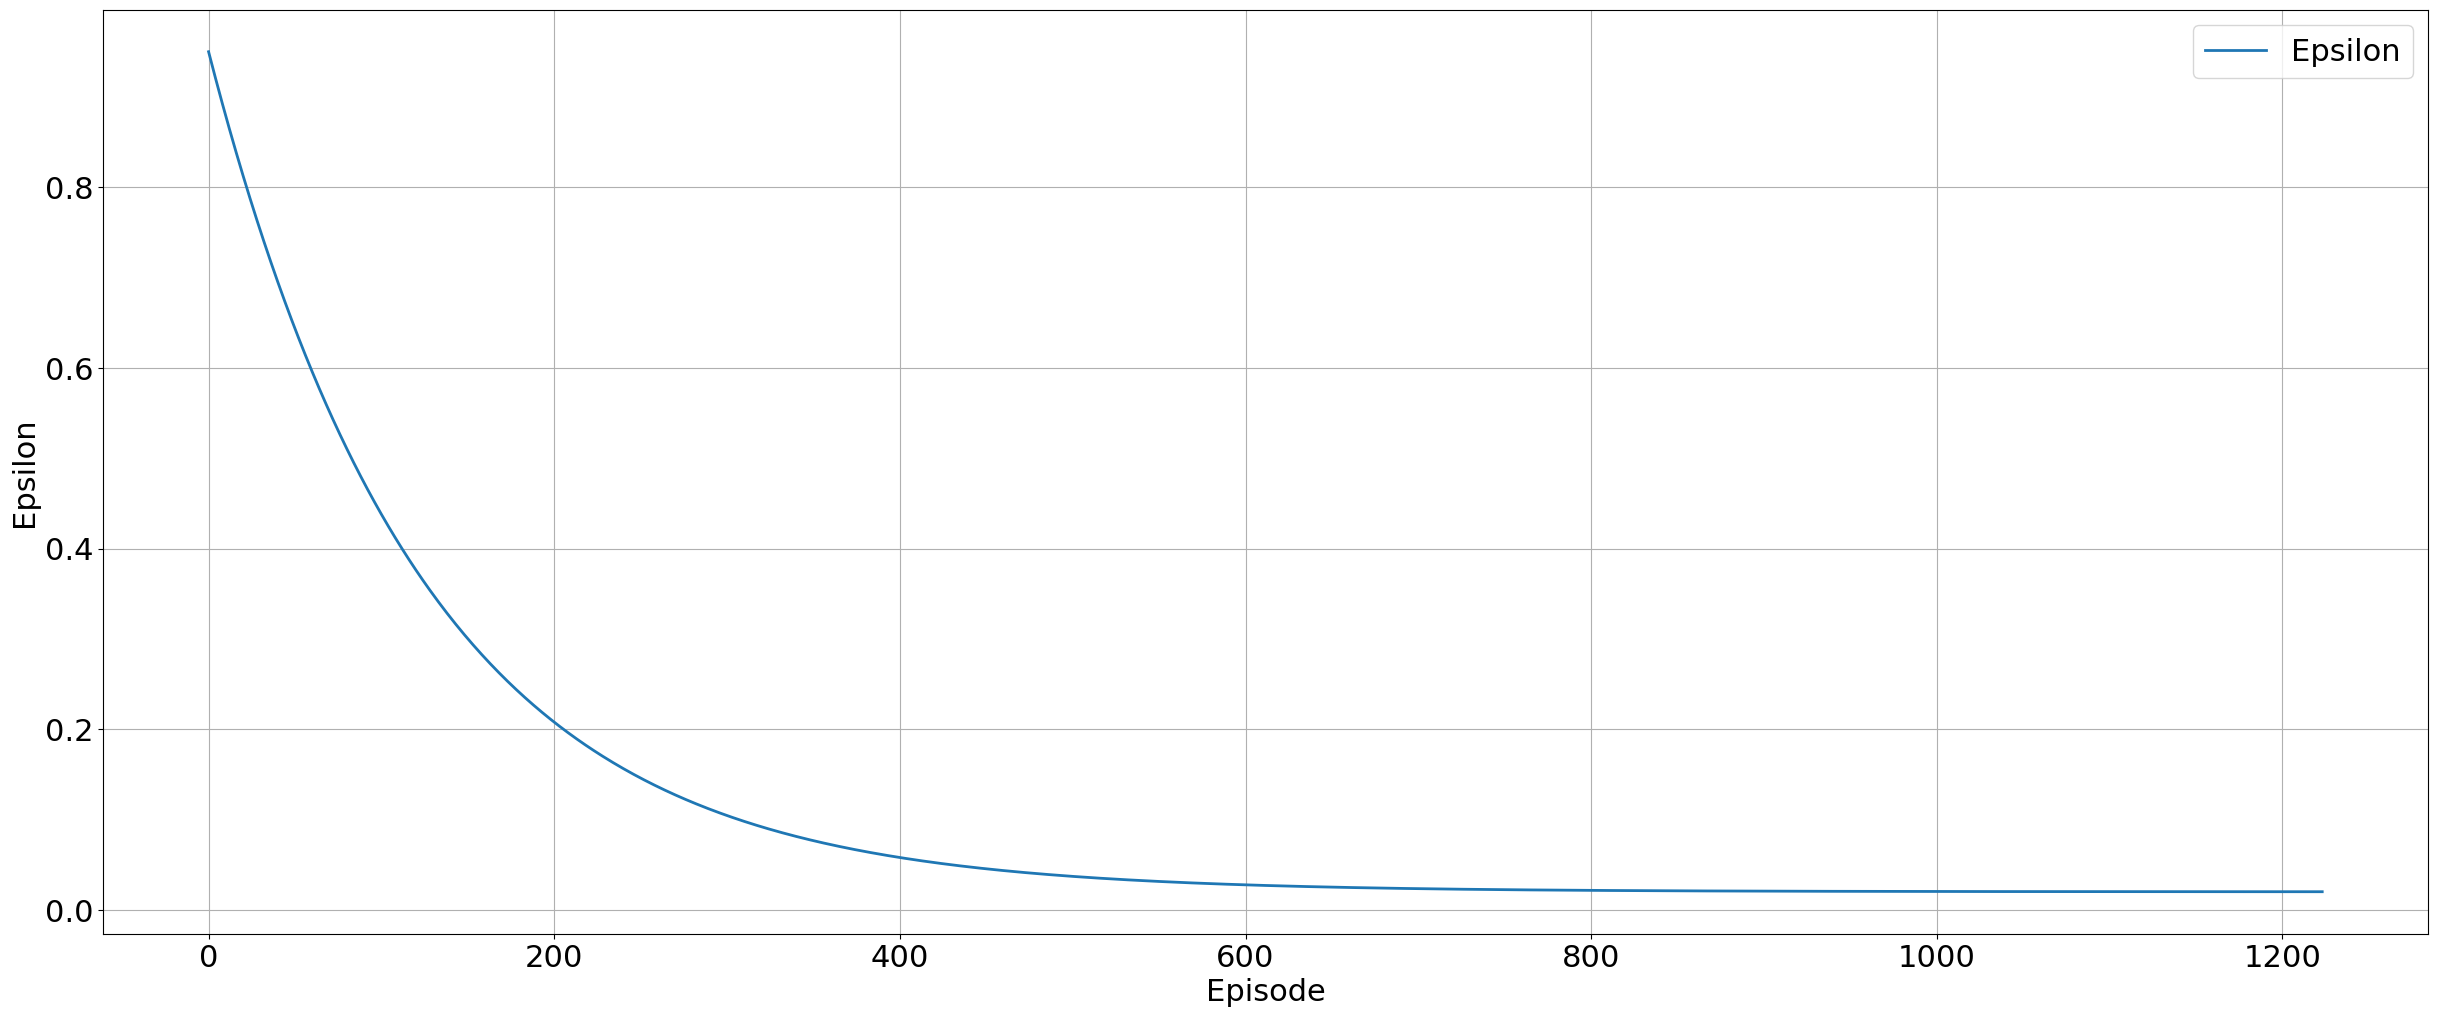
\includegraphics[width=\textwidth]{eps_lunar_ddqn.png}
    \end{center}
    \caption{Epsilon Decay -- Lunar Lander}
\end{figure}

We successfully solved all three environments using simple \verb|FeedForward| neural networks. Additionally, we implemented a tau-based Target Network update strategy to stabilize the training process and used an experience replay memory of size 10000. Of the three environments, \verb|CartPole-v1| exhibited the most unstable learning. This instability is due to the fact that a single misstep in \verb|CartPole-v1| can cause the pole to collapse and the episode to end prematurely. The other two environments had more stable learning curves and were successfully solved by the DQN agent.

\section{Provide the evaluation results. Run your agent on the three environments for at least 5 episodes, where the agent chooses only greedy actions from the learnt policy.}

\begin{figure}[H]
    \begin{center}
        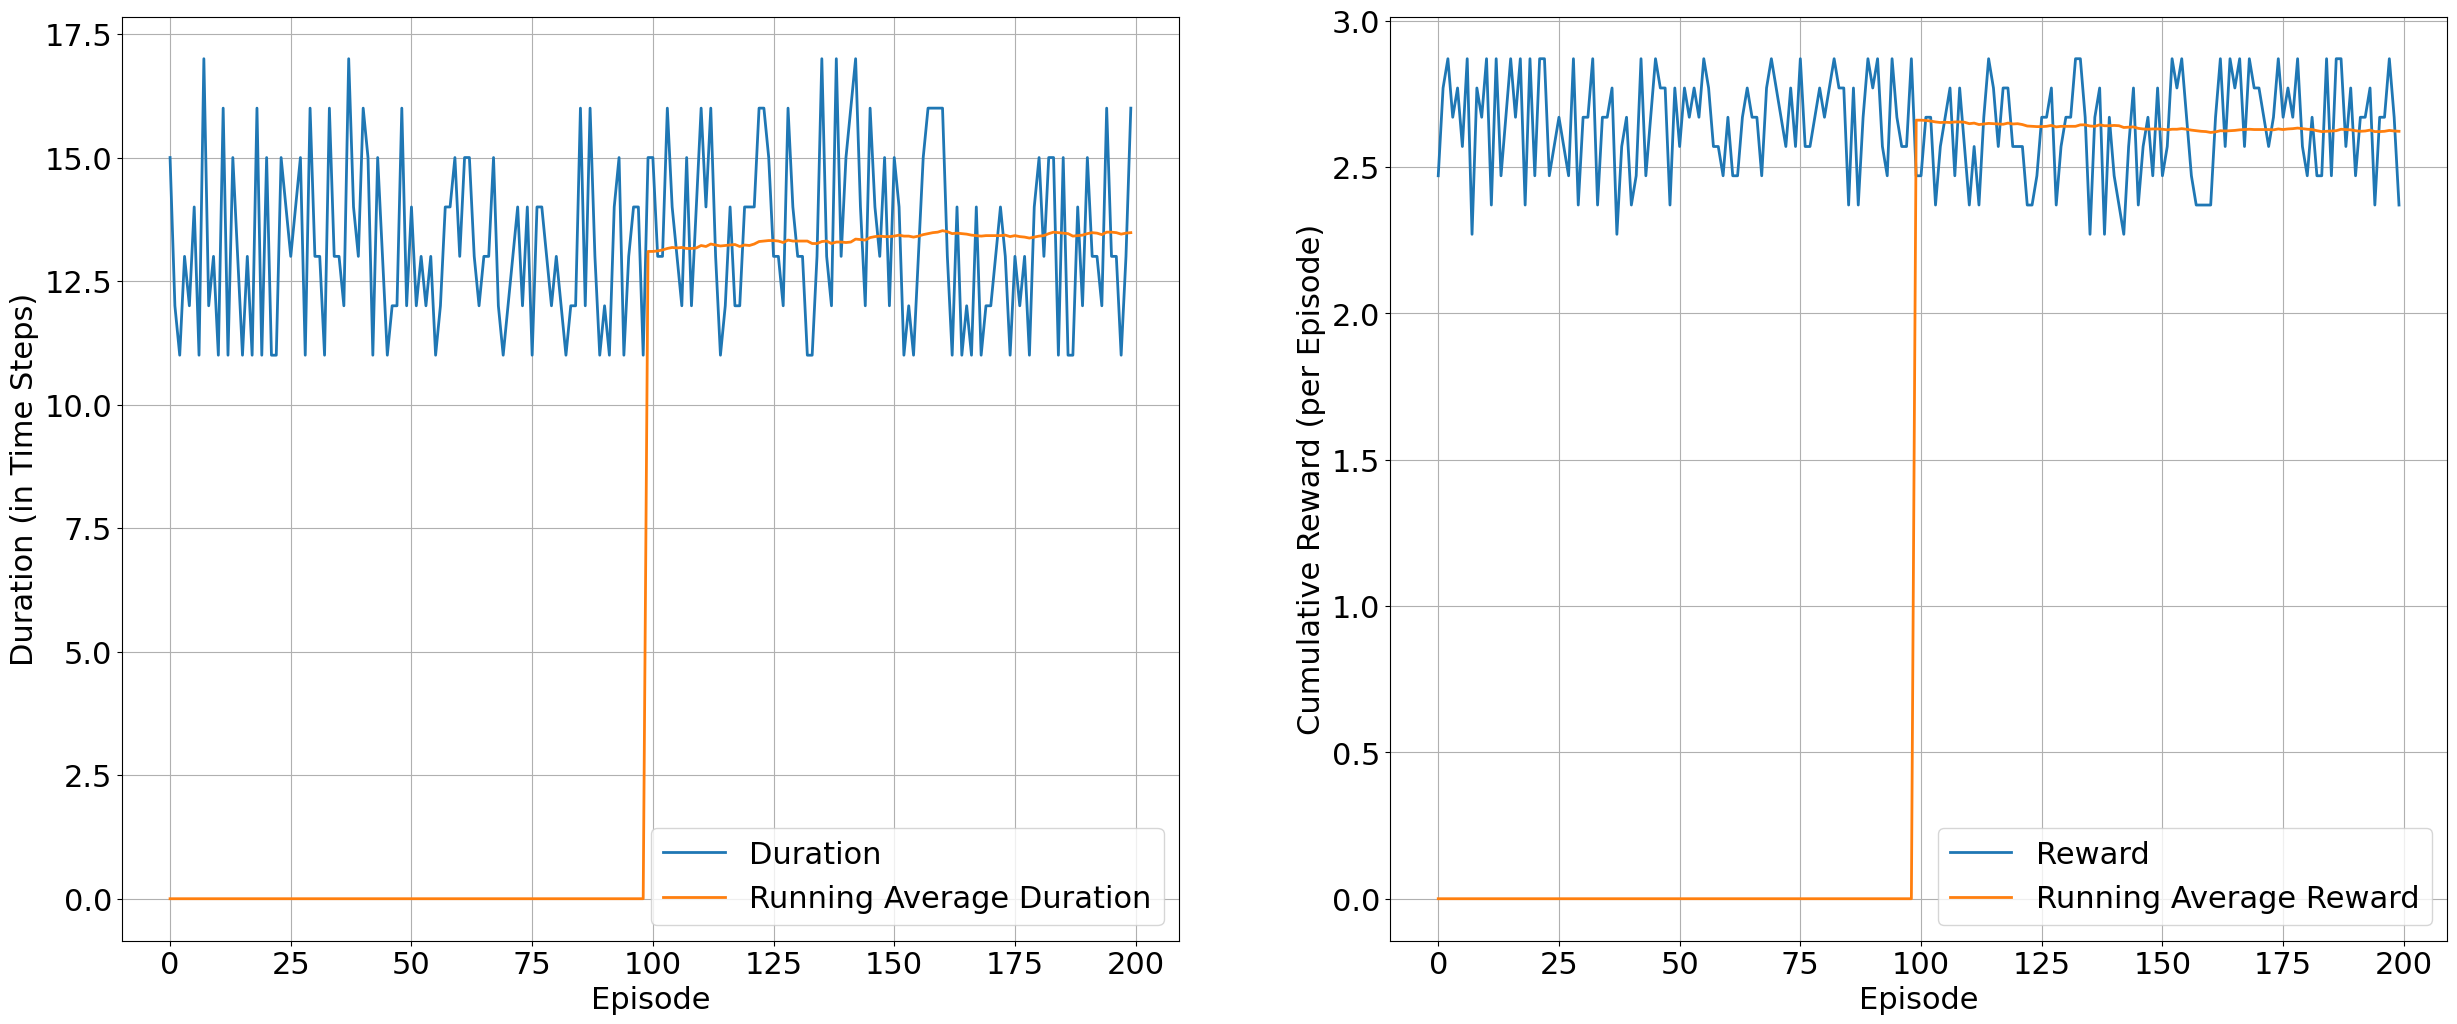
\includegraphics[width=\textwidth]{grid_evaluate.png}
    \end{center}
    \caption{Grid Environment Evaluation}
\end{figure}

\begin{figure}[H]
    \begin{center}
        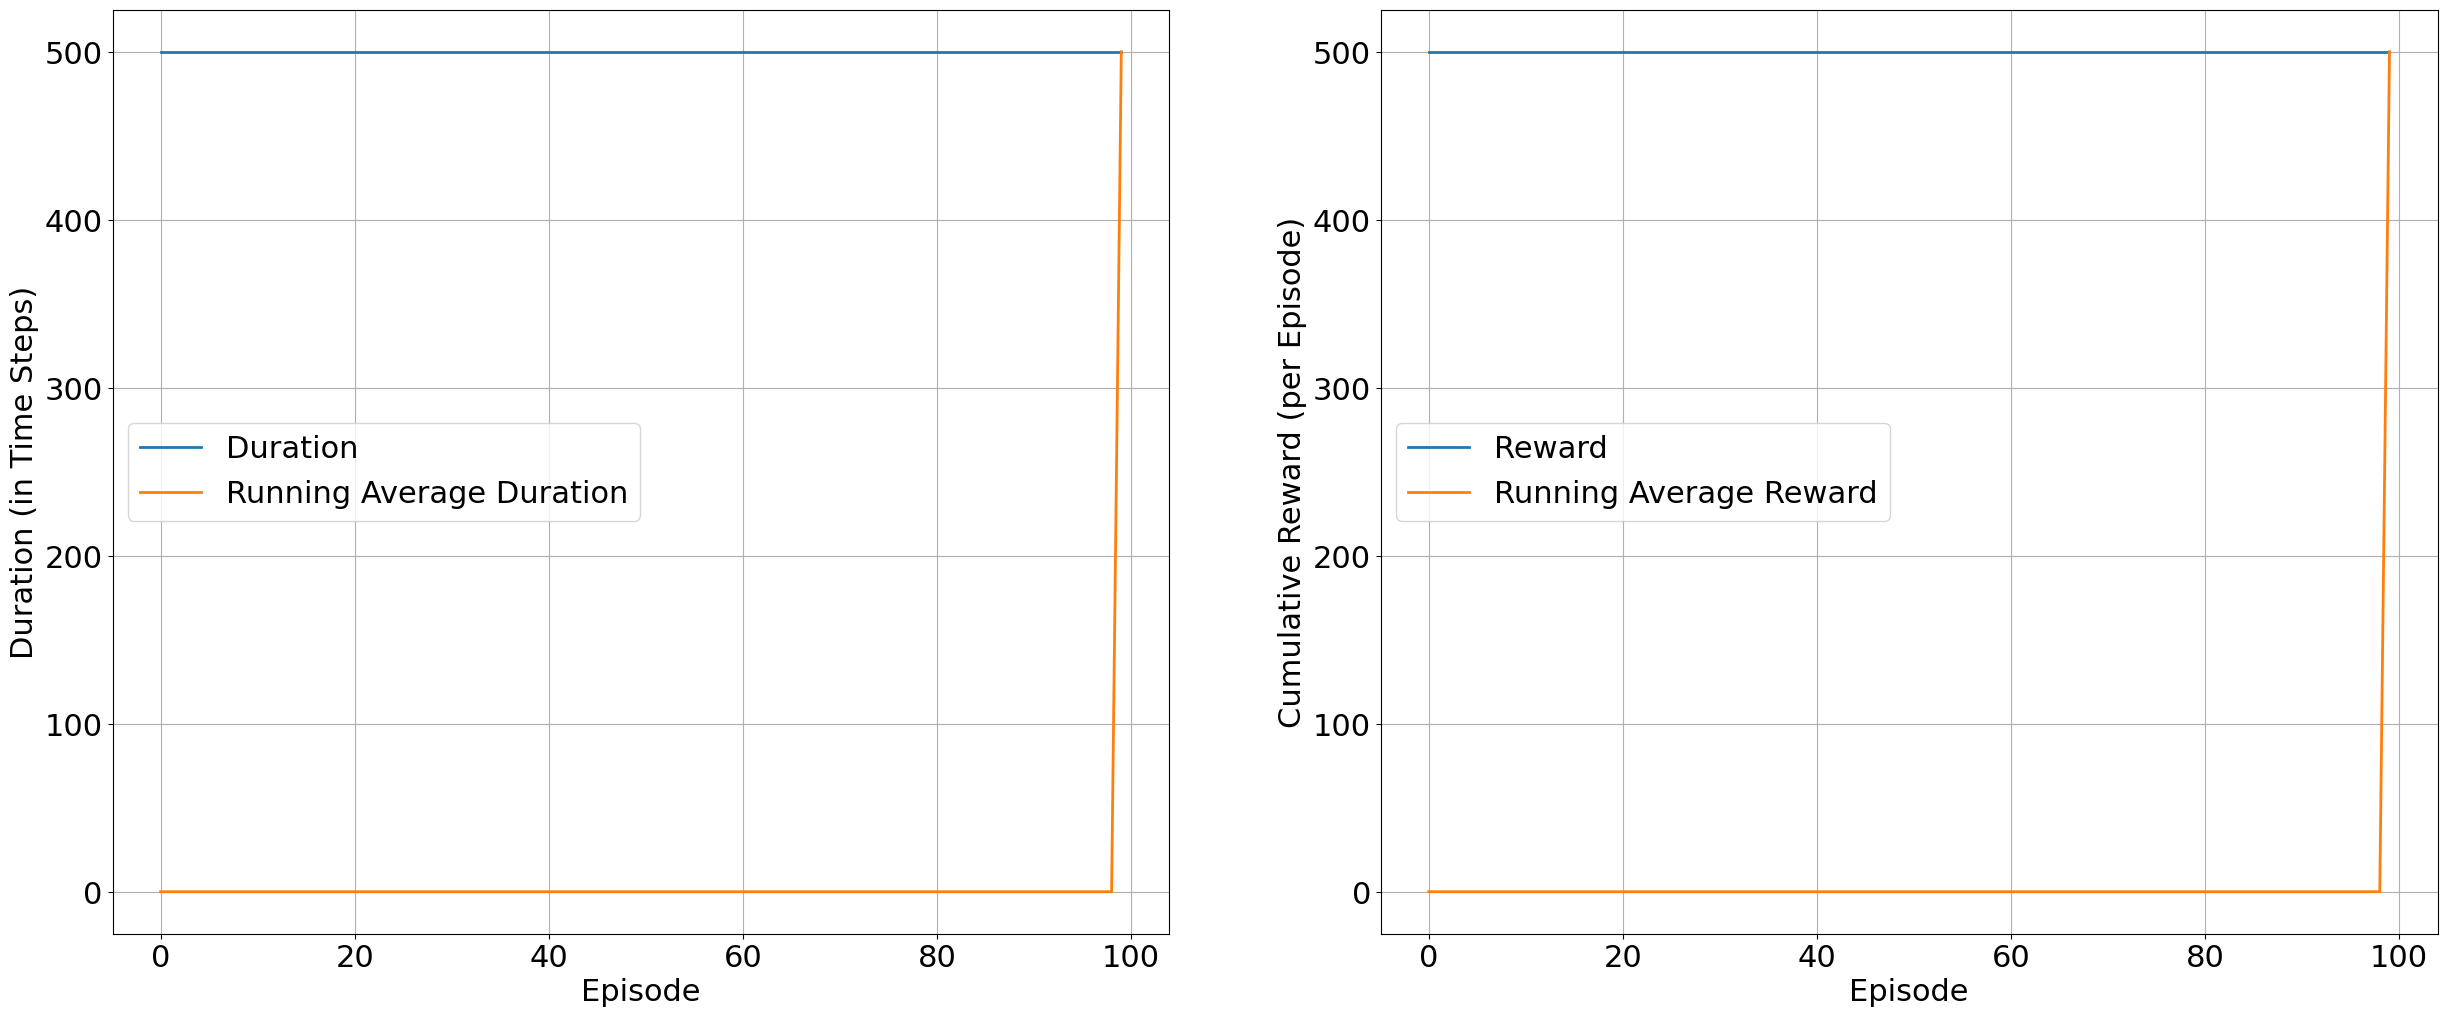
\includegraphics[width=\textwidth]{cart_evaluate.png}
    \end{center}
    \caption{Cart Environment Evaluation}
\end{figure}

\begin{figure}[H]
    \begin{center}
        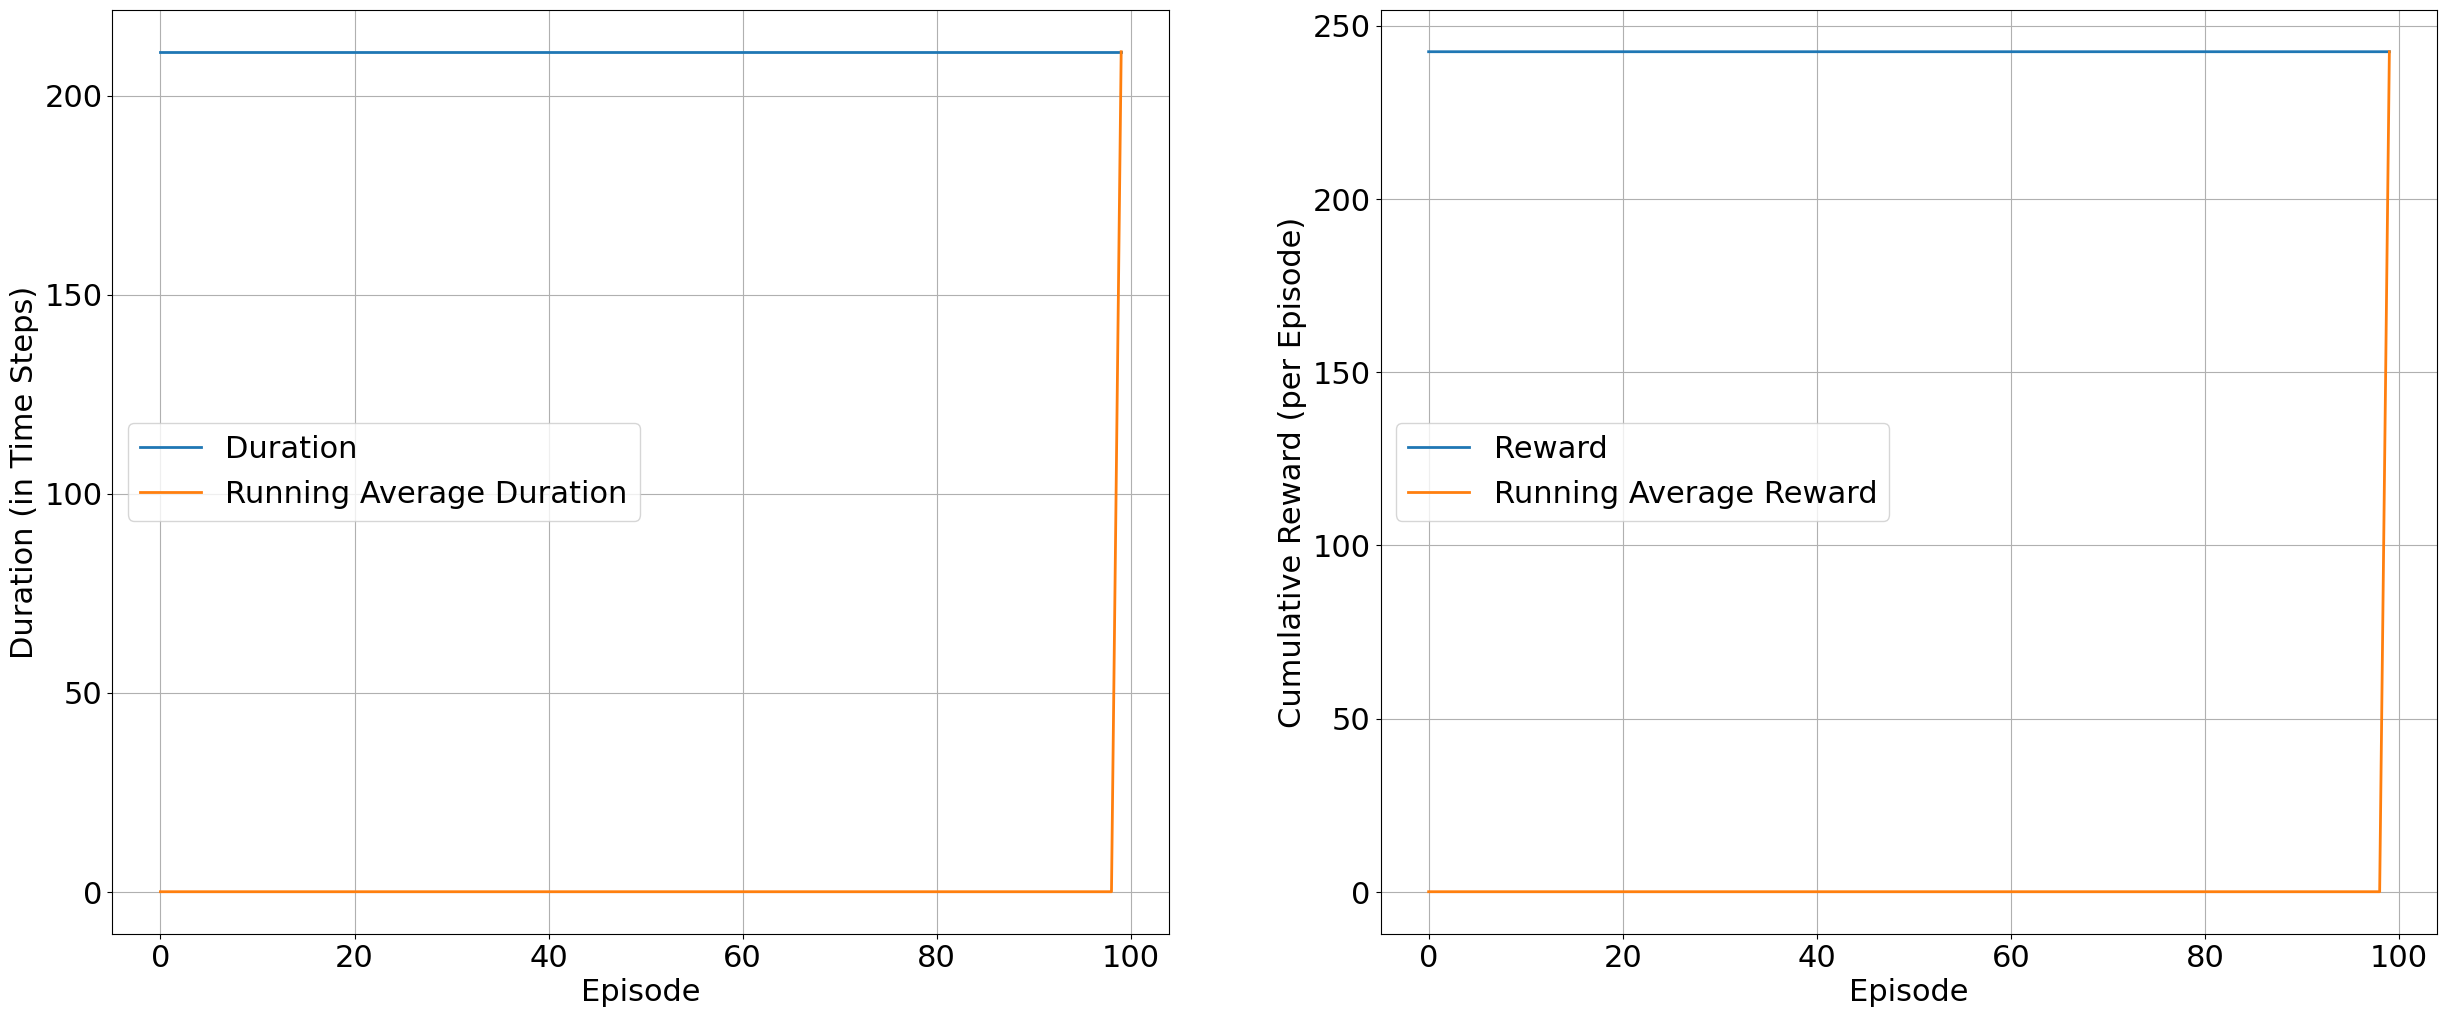
\includegraphics[width=\textwidth]{lunar_evaluate.png}
    \end{center}
    \caption{Lunar Environment Evaluation}
\end{figure}

The Deep Q-Learning \cite{mnih2013playing} with a \verb|FeedForward| neural network approach has successfully learned the optimal
policy for all three environments. The evaluation result for the GridEnvironment varies
due to the agent being placed at a random start squares, which affect the number of steps
required to reach the goal. To encourage the agent to reach the goal as quickly as possible,
we applied a negative reward of $-0.1$ for each step taken.


\section{Discuss the Double Deep Q-Learning algorithm and the main improvements over vanilla DQN.}
Double Deep Q-Network (DDQN) \cite{van2016deep} is an extension of the Deep Q-Network (DQN) algorithm, which is a deep reinforcement learning technique used to learn a policy for an agent in an environment.

In DDQN, the idea is to address the issue of overestimation of Q-values, which can occur in the original DQN algorithm. This overestimation can lead to suboptimal or even unstable policies being learned.

To address this, DDQN uses a second network (known as the "target" network) to help estimate the Q-values used to update the primary network. The target network is a copy of the primary network, but with frozen parameters that are only periodically updated. This helps to prevent the overestimation of Q-values, as the target network provides a more accurate estimate of the true Q-values.

\section{Show and discuss your results after applying your DDQN implementation on the environment.
Plots should include epsilon decay and the total reward per episode}

\subsection{GridWorld}

We represent the current state of the environment as a 36 dimensional vector of rank 1. Here each
component of the vector has one of 3 values which indicate:

\begin{itemize}
    \item[$0.5$:] Agent location
    \item[$-1.0$:] Negative reward
    \item[$0.99$:] Positive reward
    \item[$1.0$:] Goal square
\end{itemize}

We feed this vector to a \verb|Feed-forward Network| that will give us the estimated
action-values. Then We take the \verb|argmax| over these action-values. We consider the
environments as solved when we have achieved a 100 episode running average of $~2.1$.

\subsection{CartPole-v1 \& LunarLander-v2}
For both these environments we have rather similar action spaces (\verb|Discrete|), hence the
\verb|Feed-forward Network| architechture used is also similar. The input of the network has the shape
\verb|1 x state-space| output of network will \verb|1 x action-space|.

The enivironments are considered solved when:
\begin{itemize}
    \item[] \textbf{CartPole-v1} Running average reward of 500 (100 episodes)
    \item[] \textbf{LunarLander-v2} Running average reward $>$ 200 (100 episodes)
\end{itemize}



\subsection{Training Discussion}

\begin{figure}[H]
    \begin{center}
        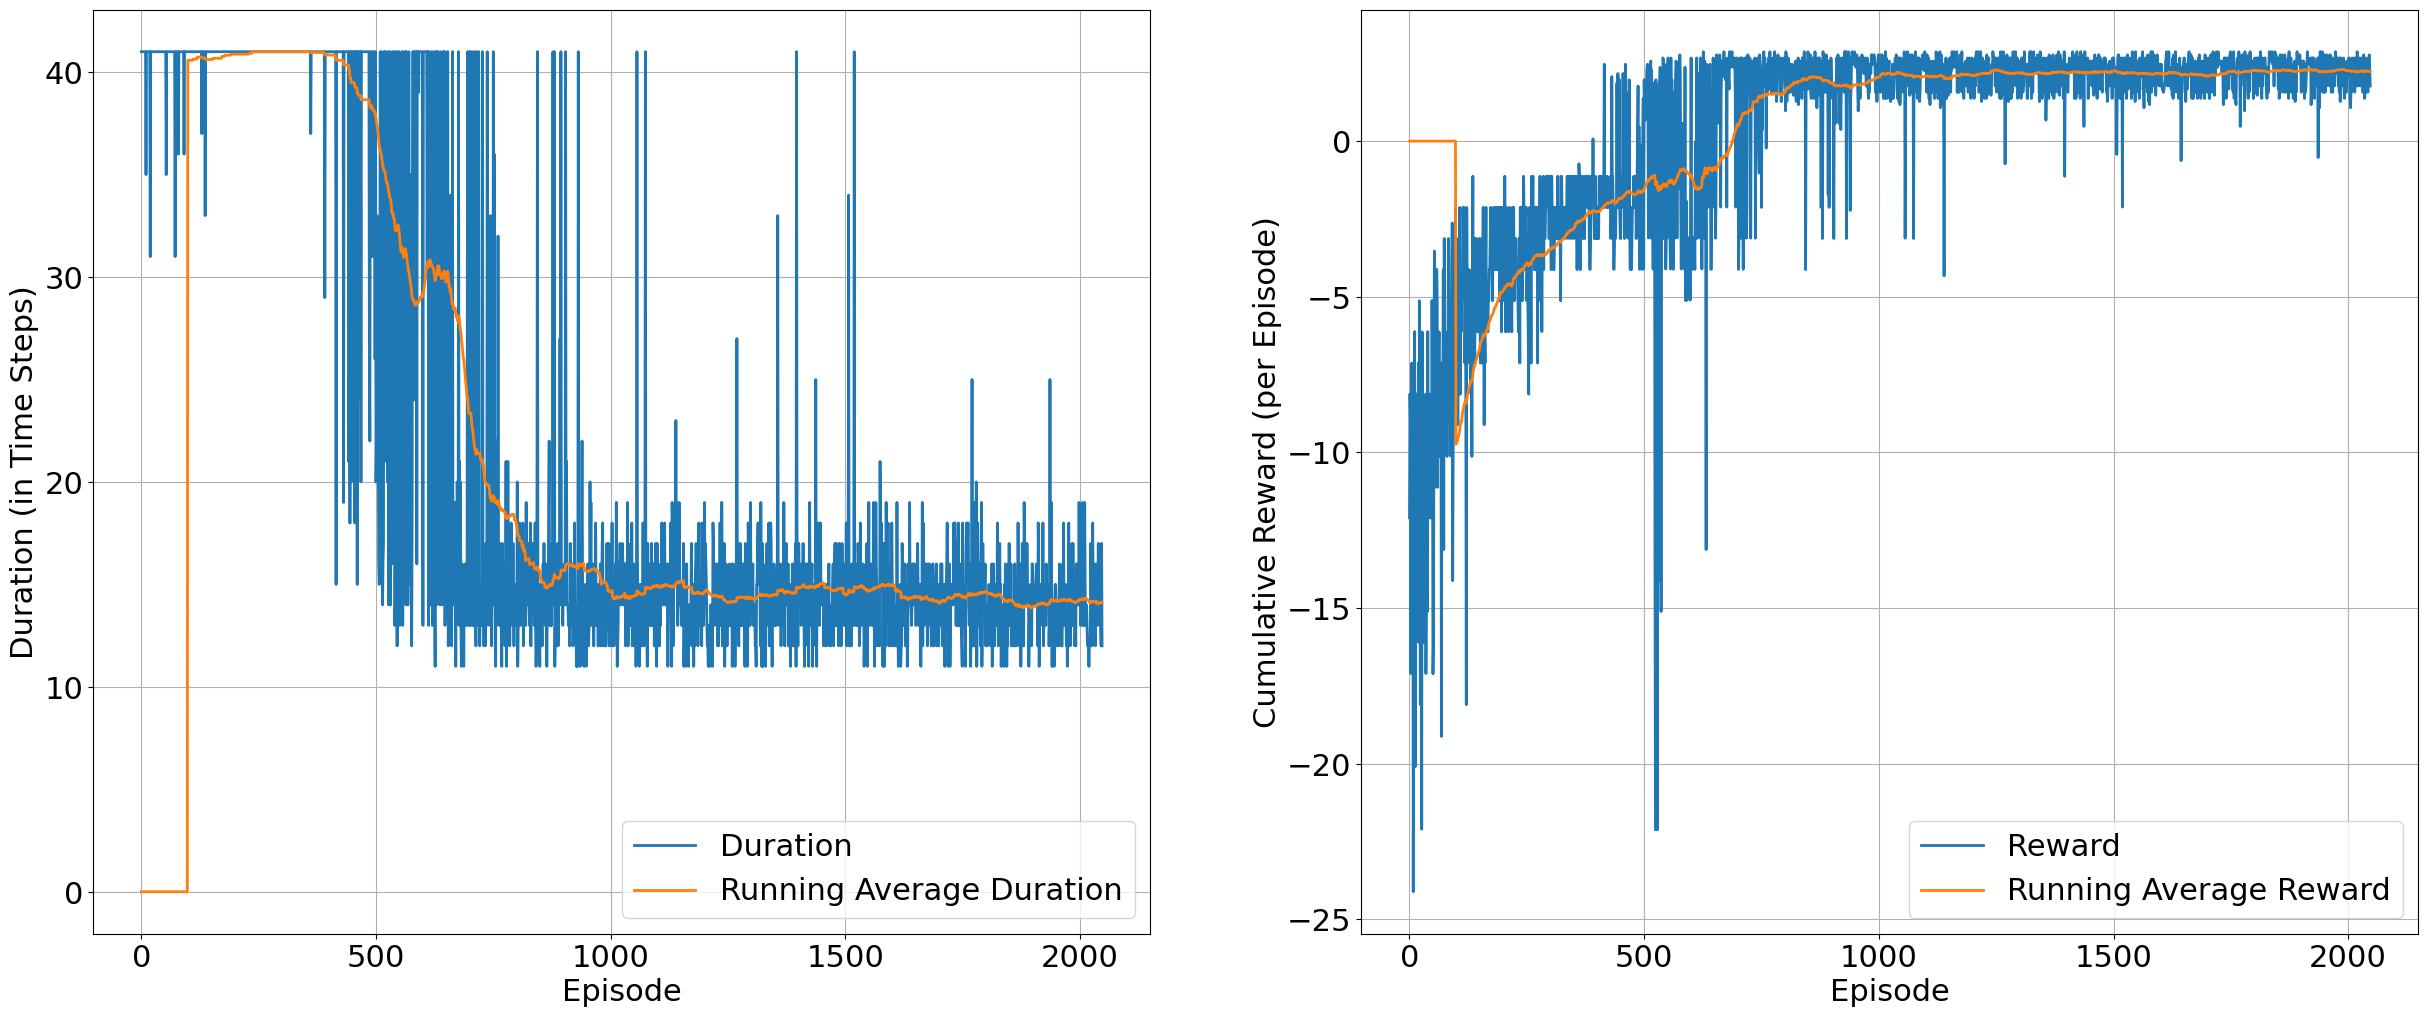
\includegraphics[width=\textwidth]{grid_training_ddqn.png}
    \end{center}
    \caption{Grid Training}
\end{figure}

\begin{figure}[H]
    \begin{center}
        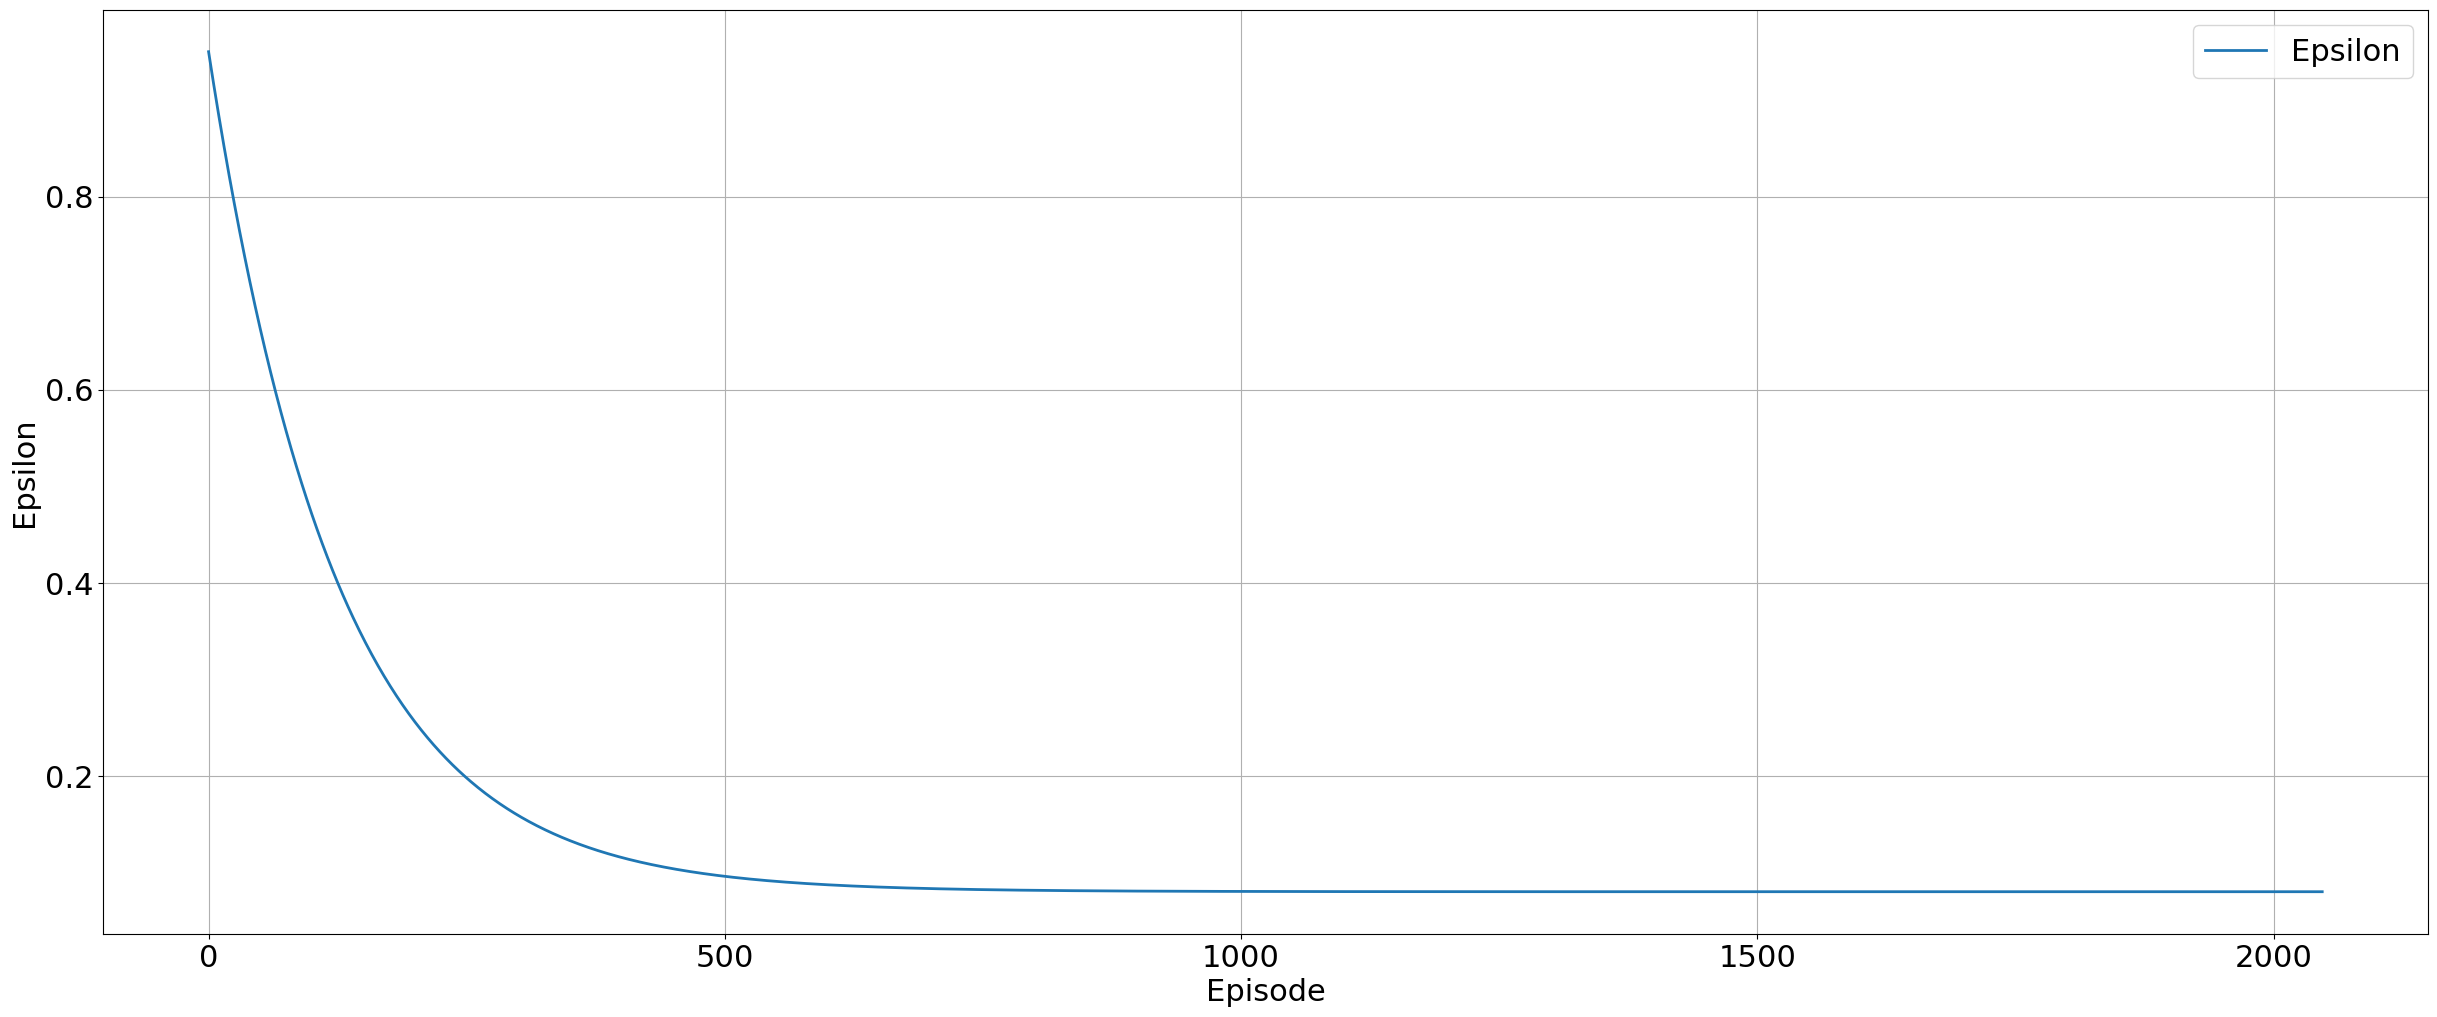
\includegraphics[width=\textwidth]{eps_grid_ddqn.png}
    \end{center}
    \caption{Epsilon Decay -- Grid Env}
\end{figure}

\begin{figure}[H]
    \begin{center}
        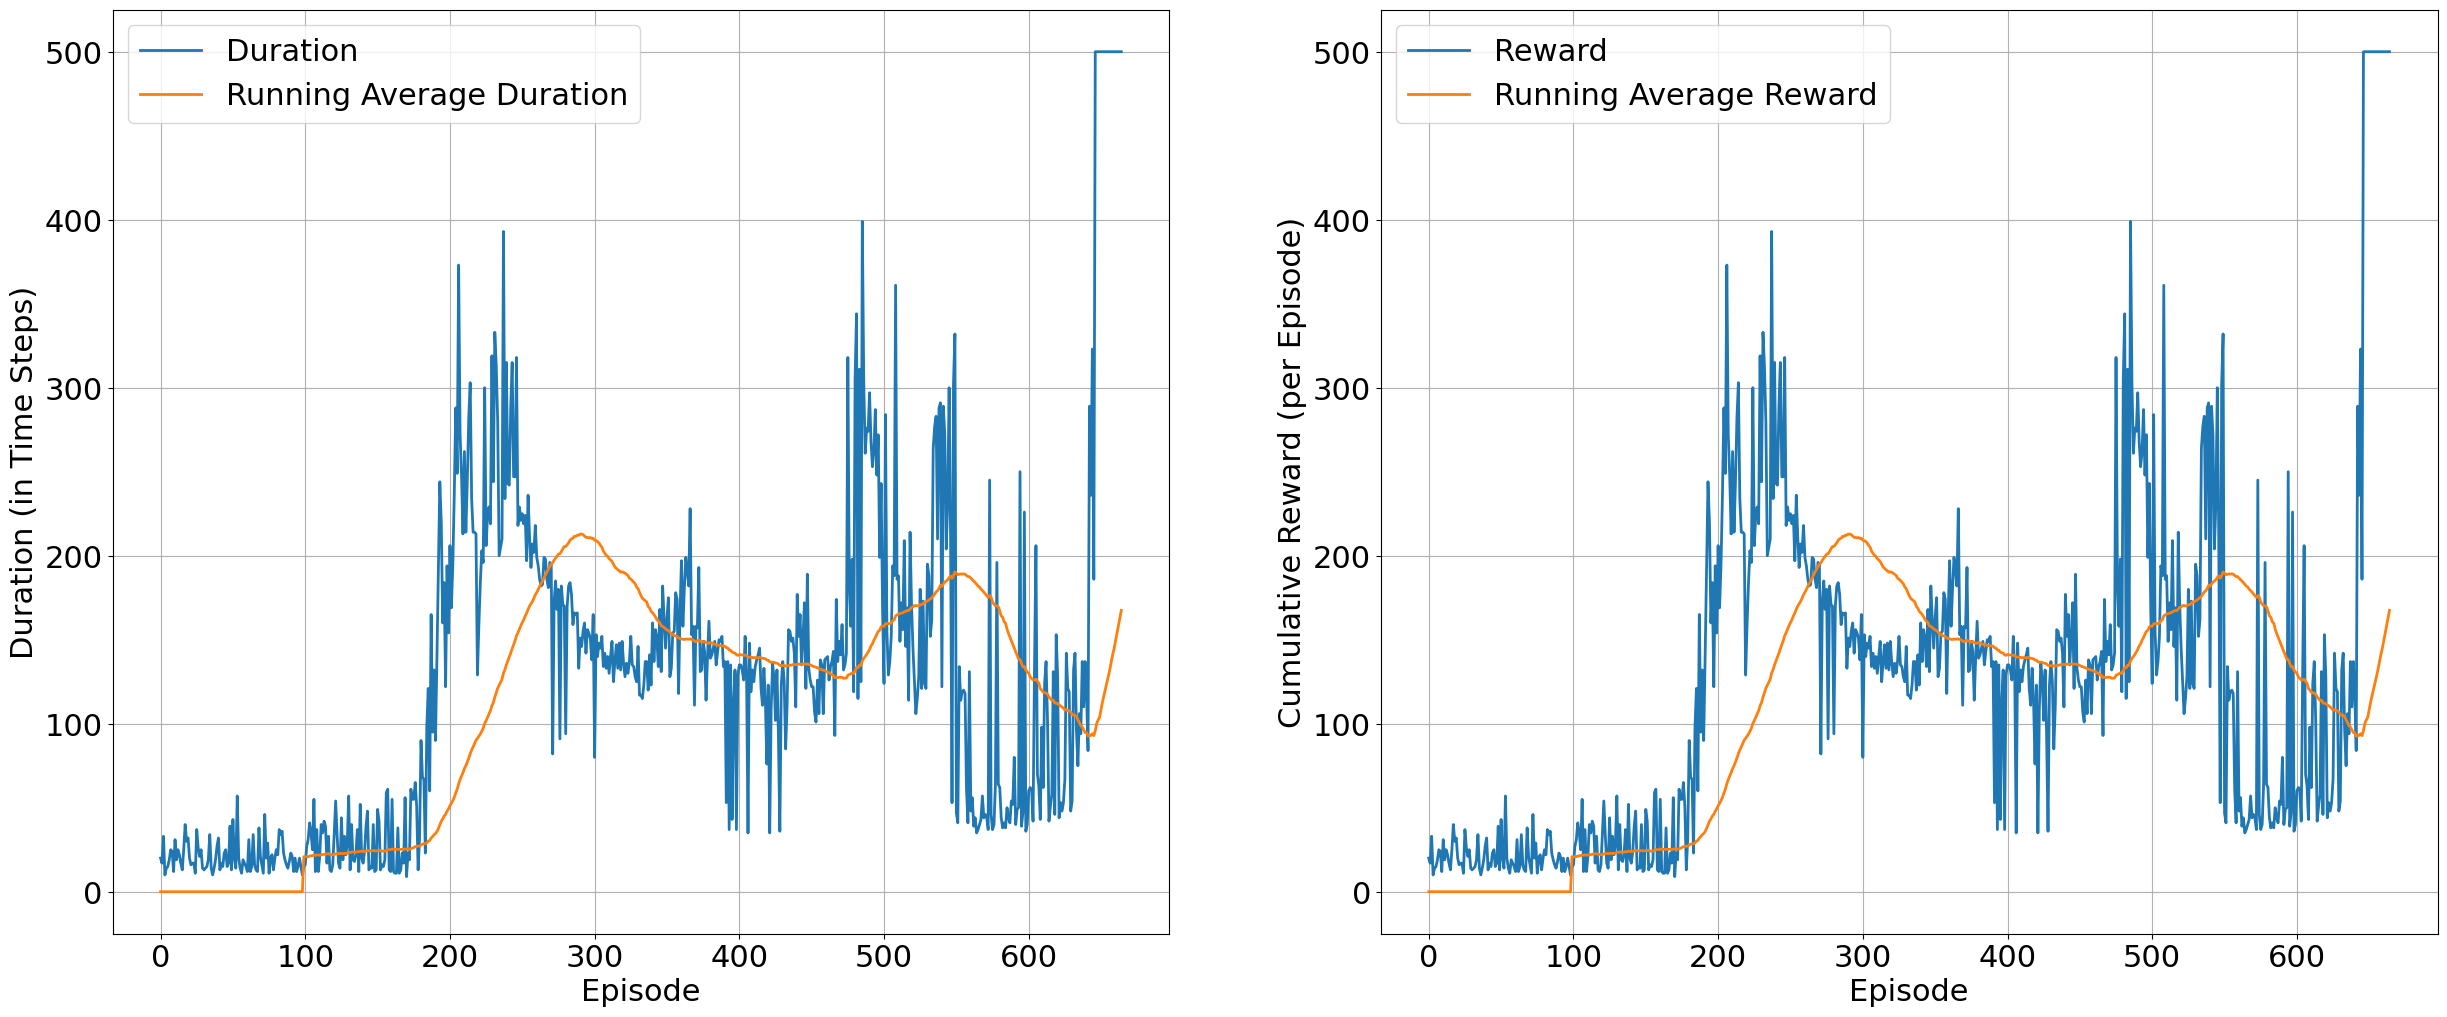
\includegraphics[width=\textwidth]{cartpole_training_ddqn.png}
    \end{center}
    \caption{Cart-Pole Training}
\end{figure}

\begin{figure}[H]
    \begin{center}
        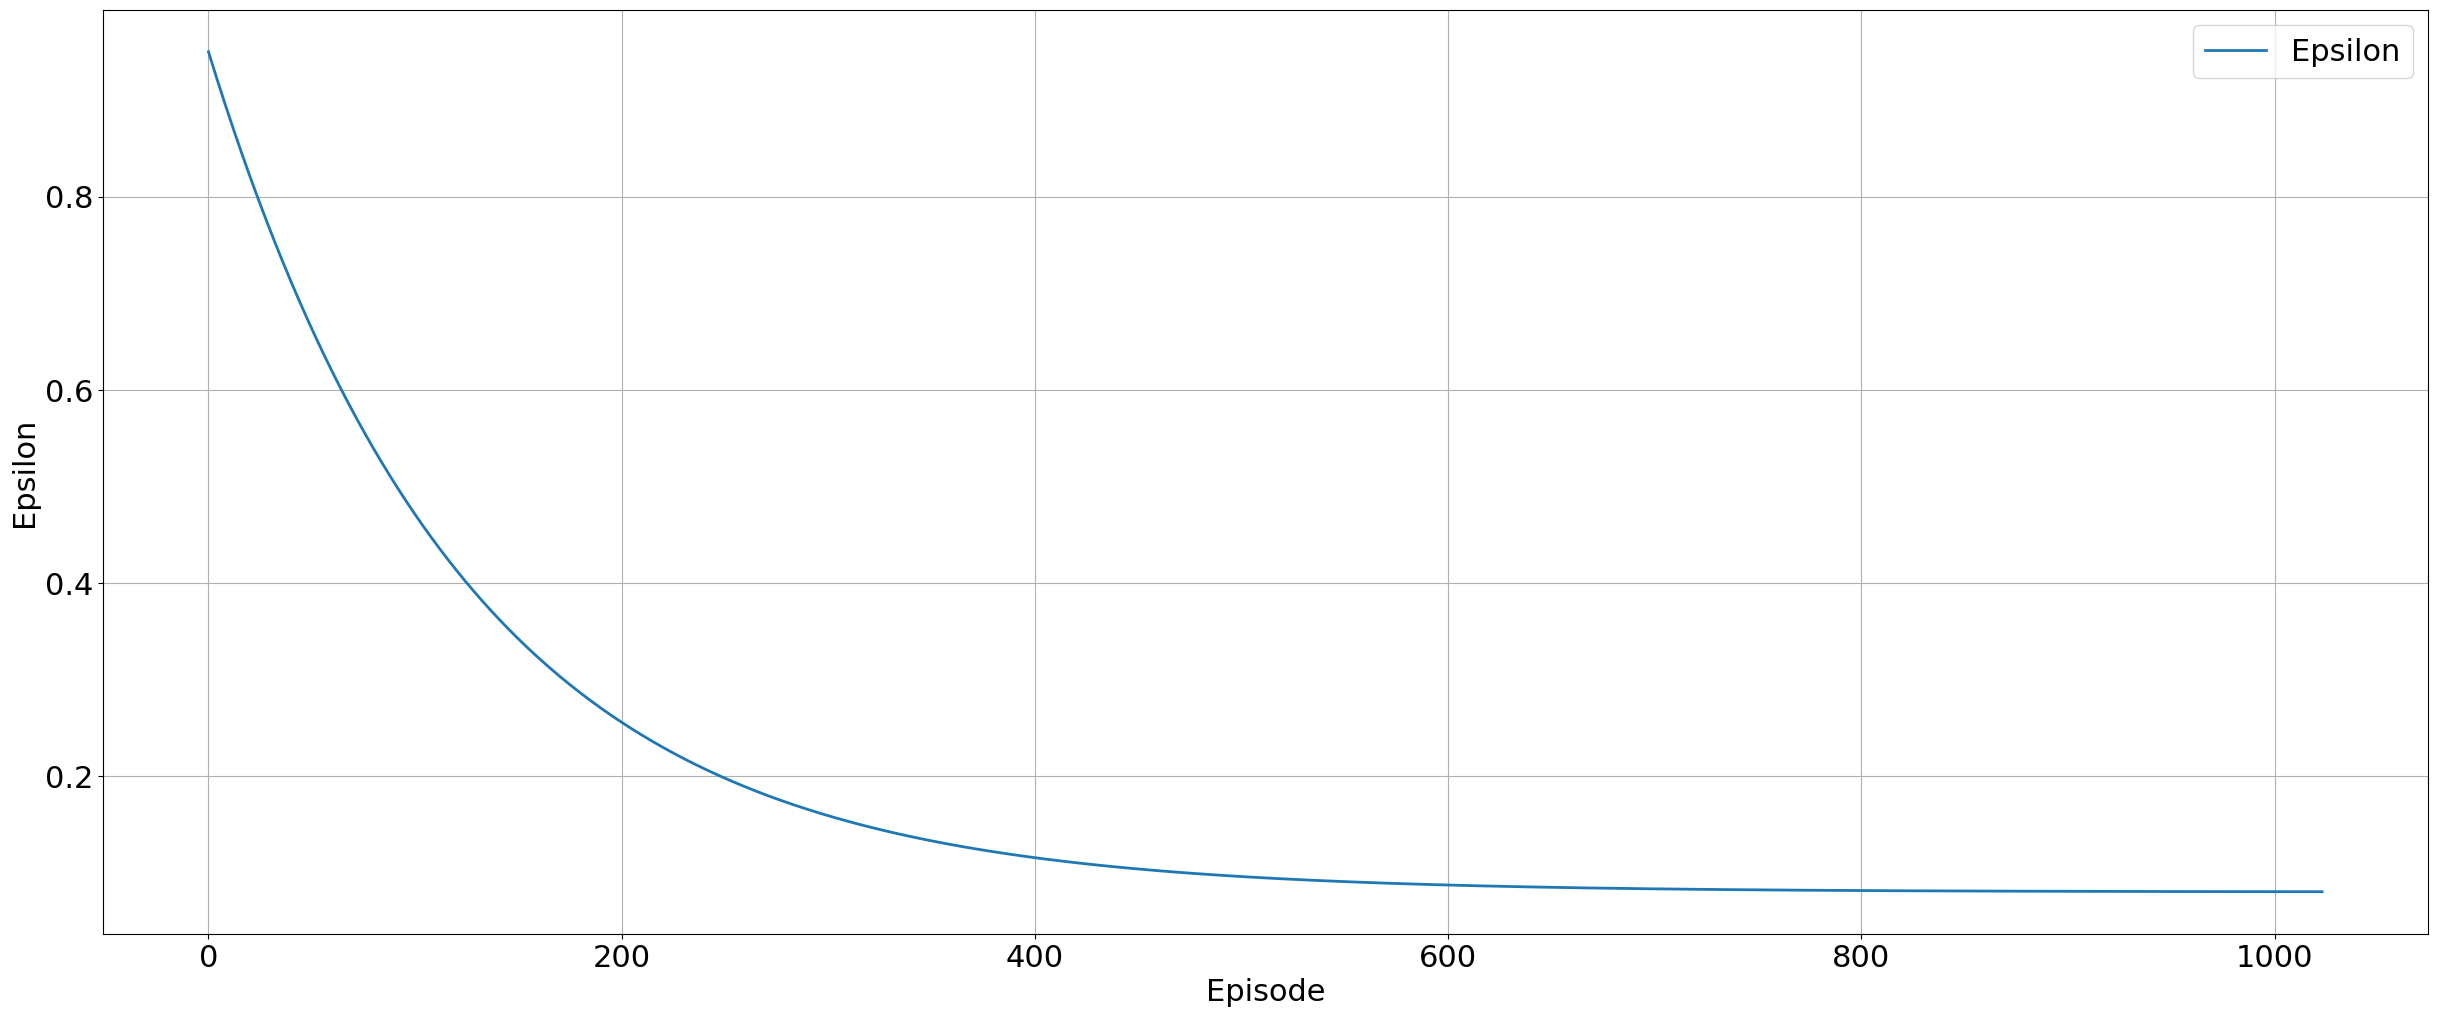
\includegraphics[width=\textwidth]{eps_cart.png}
    \end{center}
    \caption{Epsilon Decay -- Cart Pole}
\end{figure}

\begin{figure}[H]
    \begin{center}
        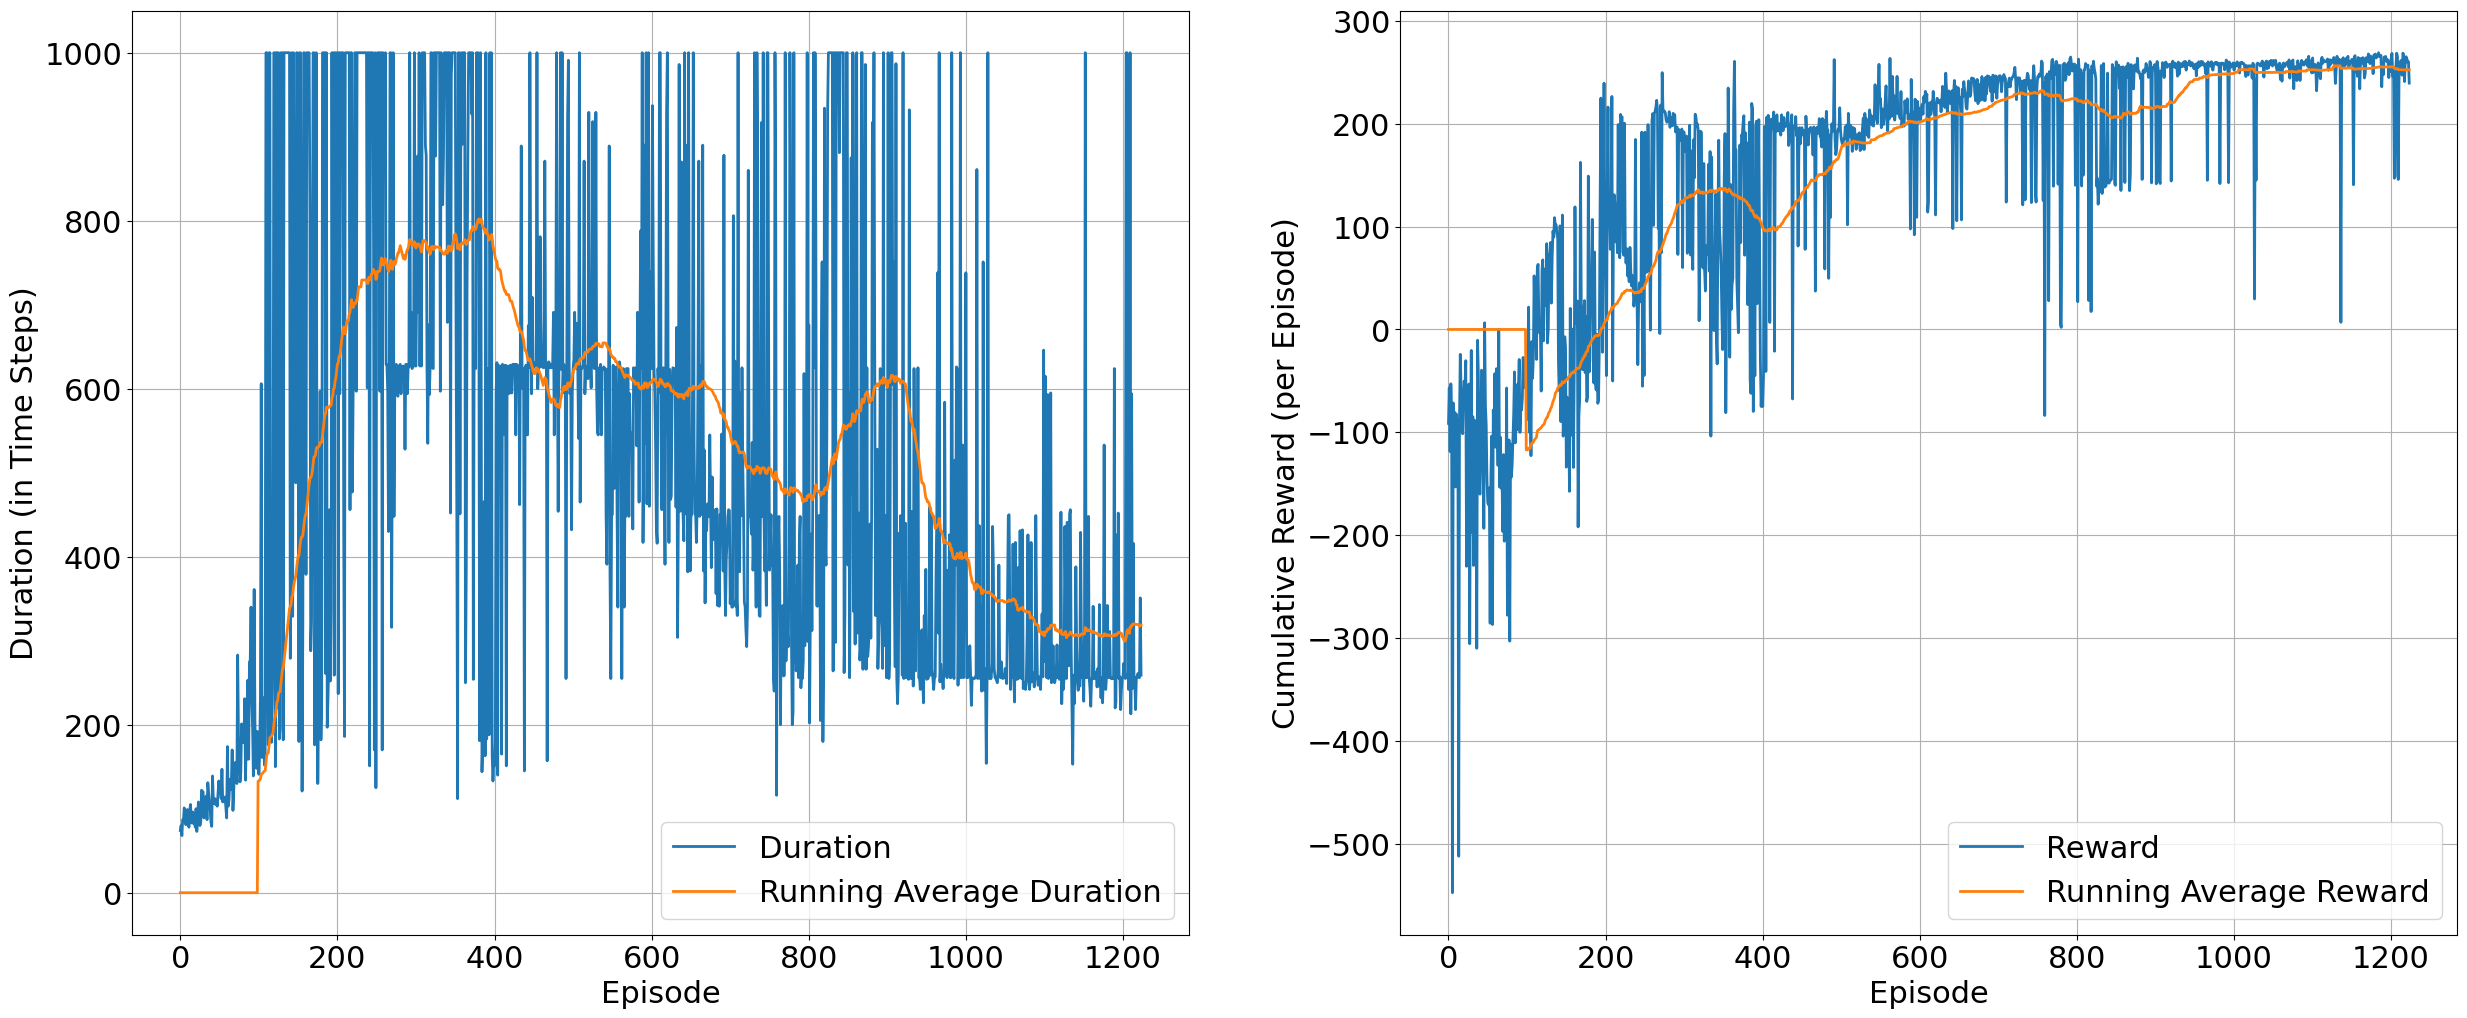
\includegraphics[width=\textwidth]{lunar_training_ddqn.png}
    \end{center}
    \caption{Lunar Lander Training}
\end{figure}

\begin{figure}[H]
    \begin{center}
        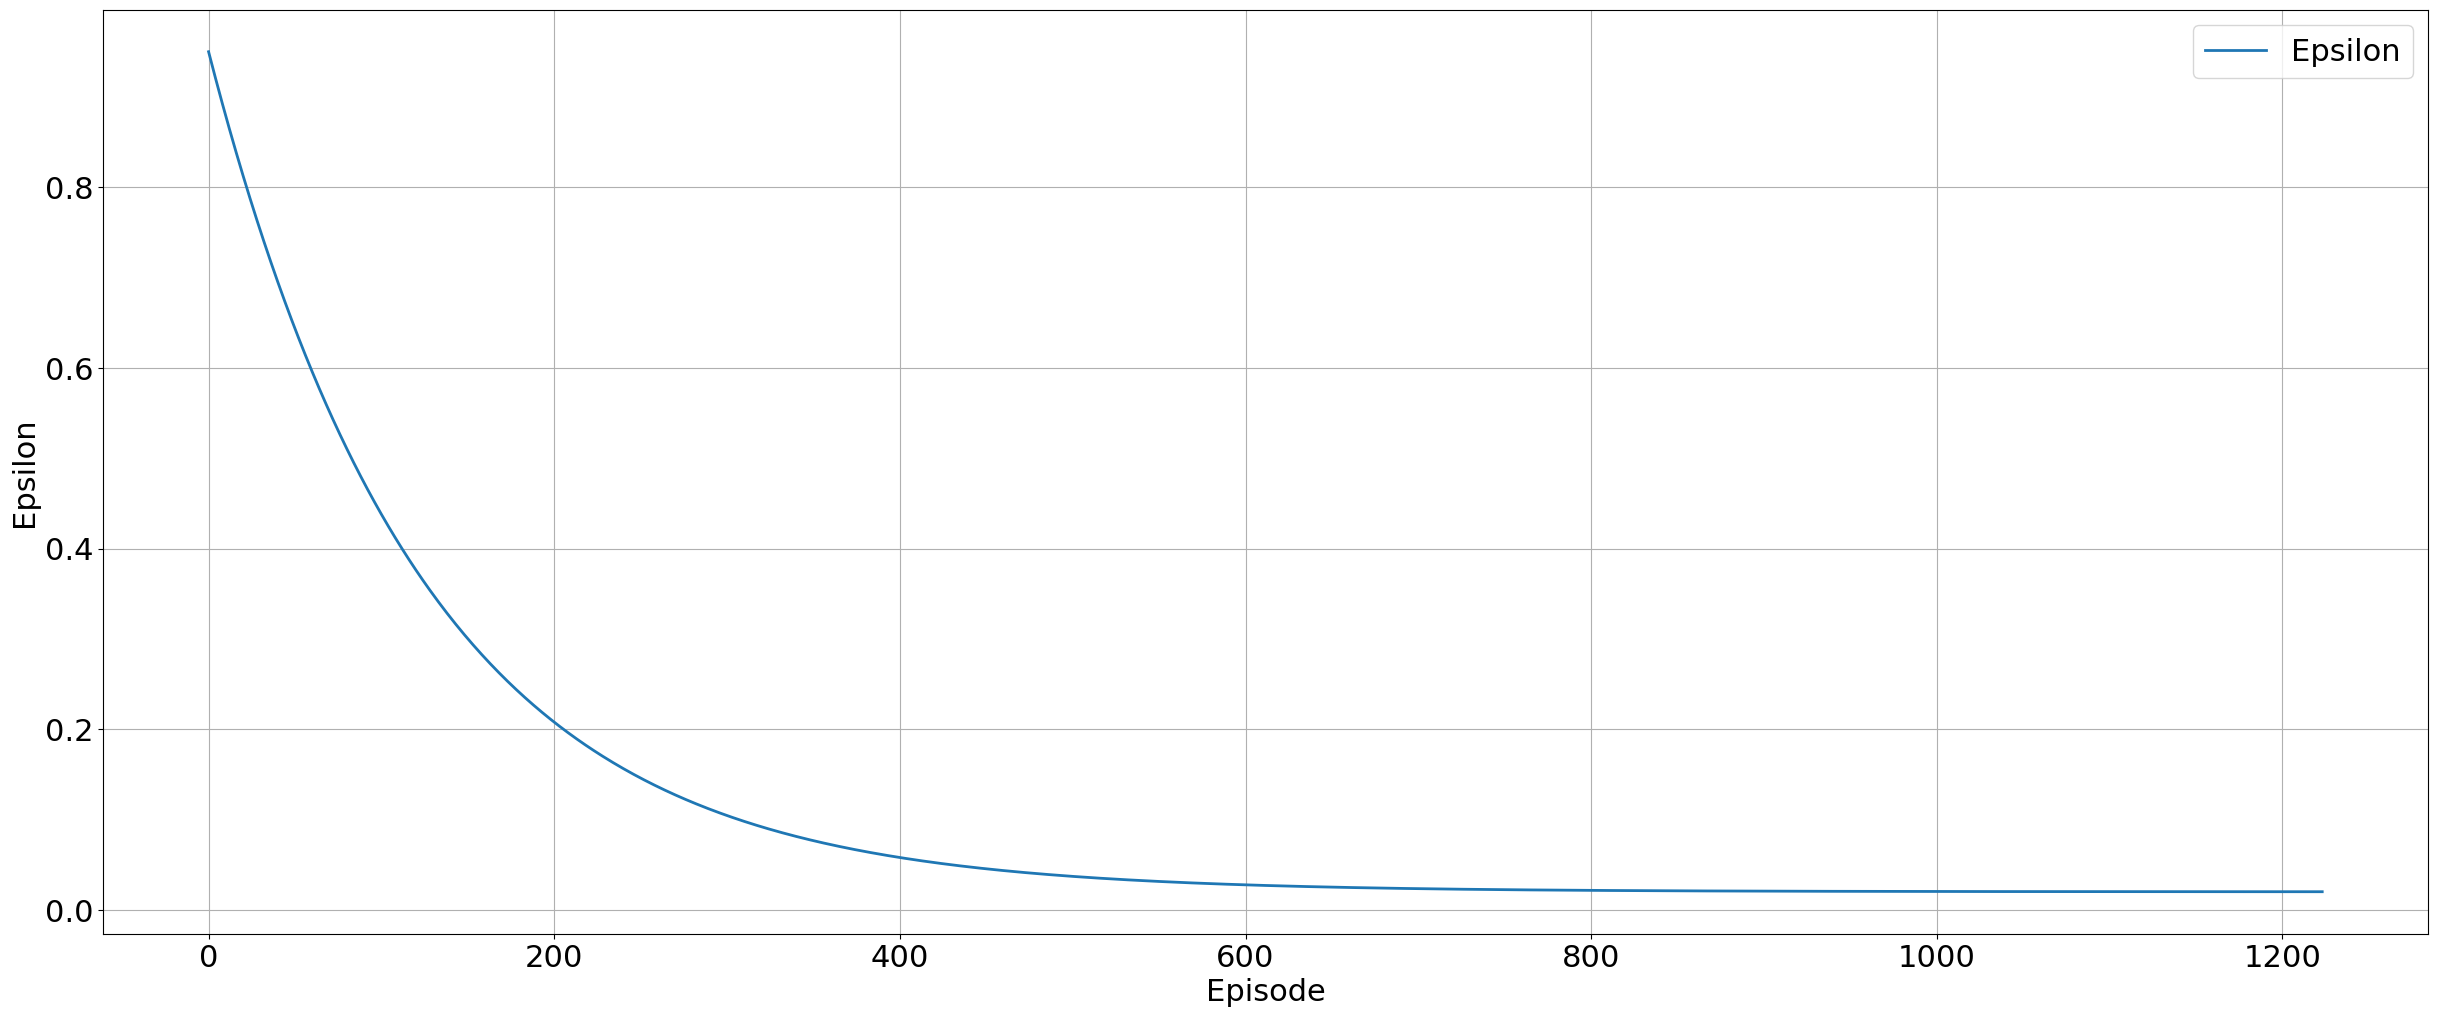
\includegraphics[width=\textwidth]{eps_lunar_ddqn.png}
    \end{center}
    \caption{Epsilon Decay -- Lunar Lander}
\end{figure}

We successfully solved all three environments using simple \verb|FeedForward| neural networks. Additionally, we implemented a tau-based Target Network update strategy to stabilize the training process and used an experience replay memory of size 10000. Of the three environments, \verb|CartPole-v1| exhibited the most unstable learning. This instability is due to the fact that a single misstep in \verb|CartPole-v1| can cause the pole to collapse and the episode to end prematurely. The other two environments had more stable learning curves and were successfully solved by the DQN agent.

\section{Provide the evaluation results. Run your agent on the three environments for at least 5 episodes, where the agent chooses only greedy actions from the learnt policy.}

\begin{figure}[H]
    \begin{center}
        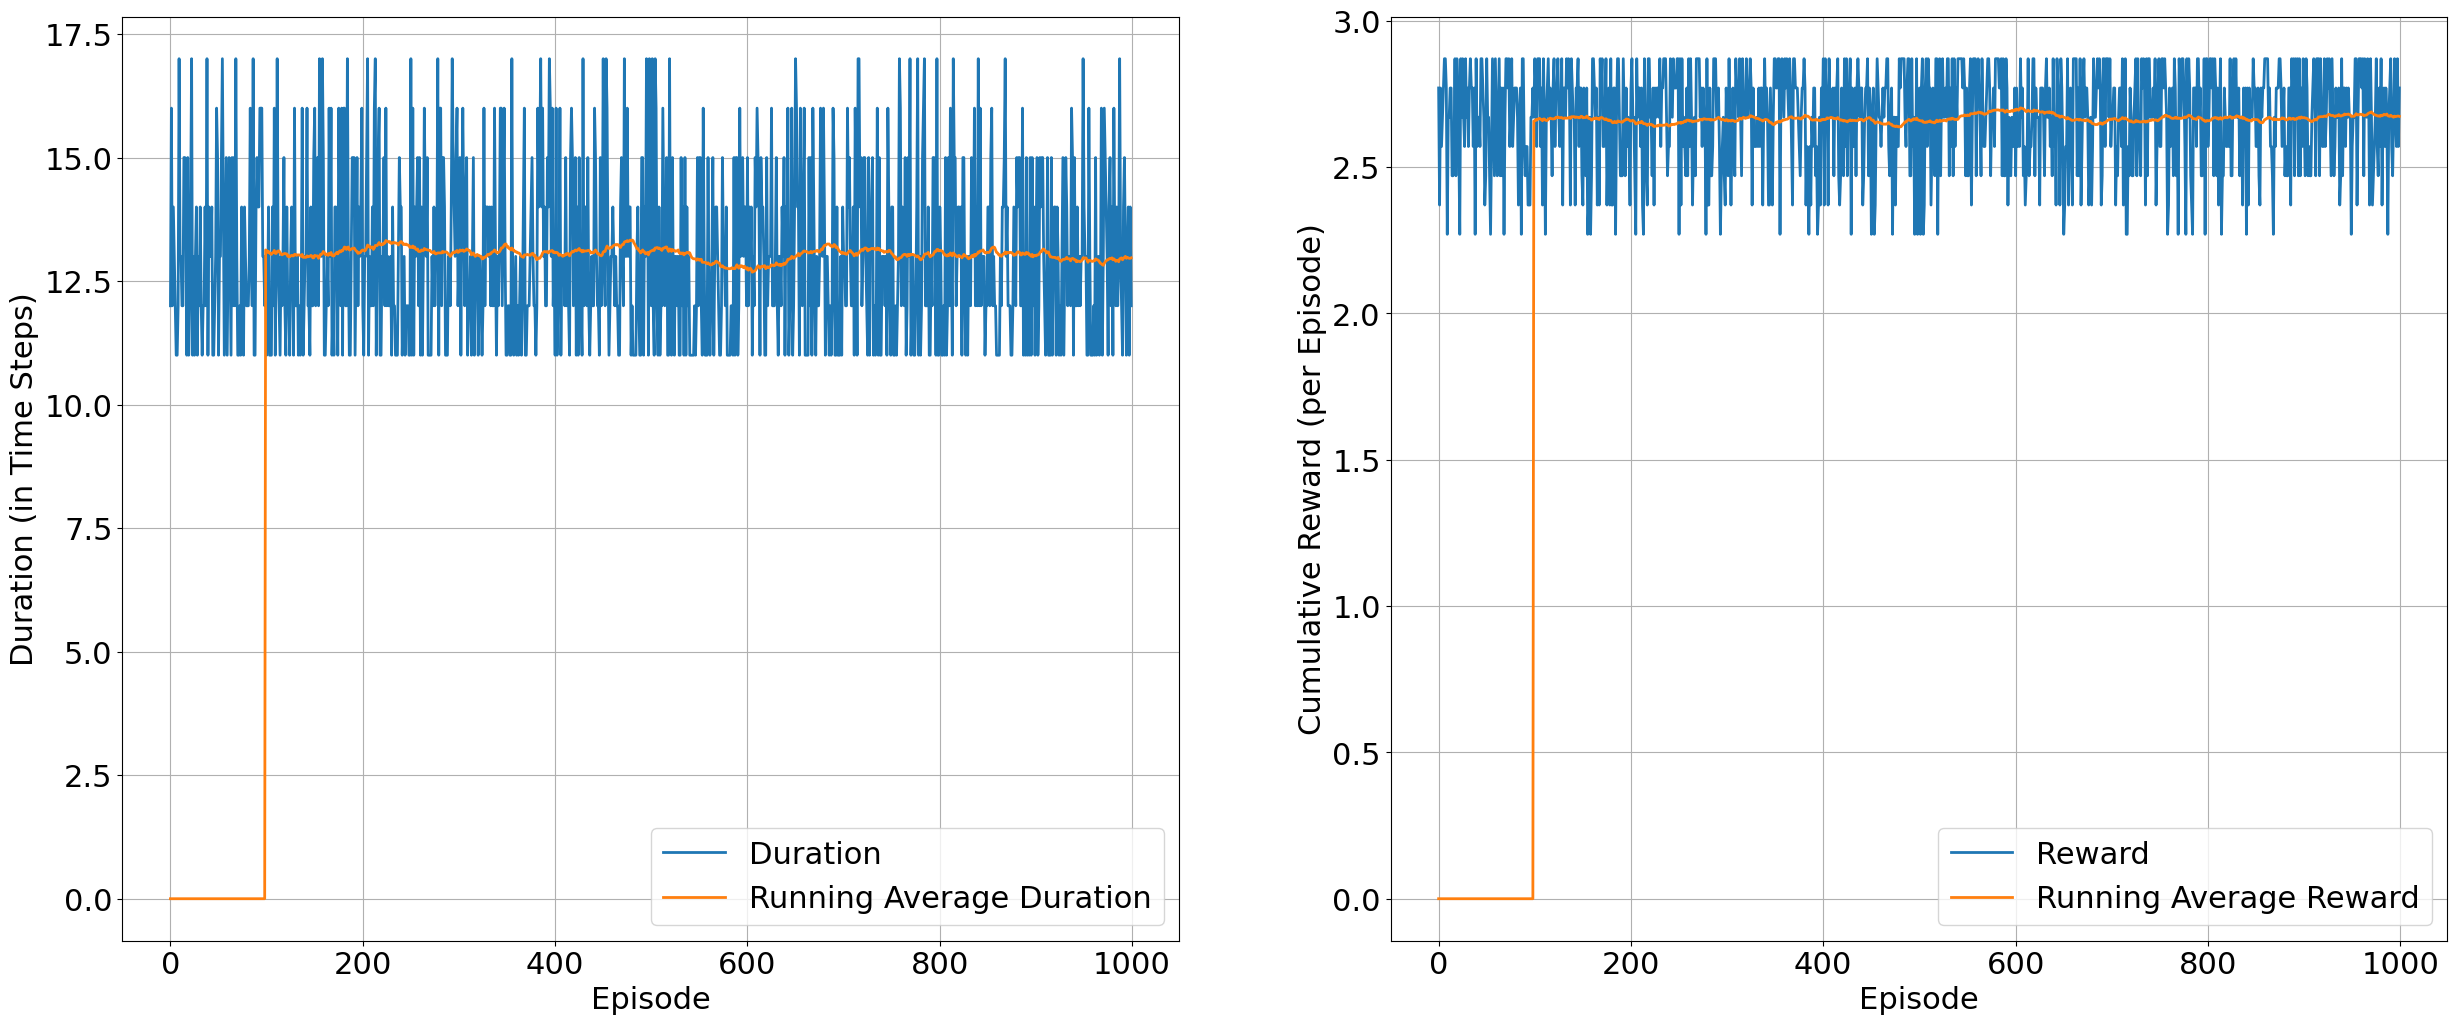
\includegraphics[width=\textwidth]{grid_evaluate_ddqn.png}
    \end{center}
    \caption{Grid Environment Evaluation}
\end{figure}

\begin{figure}[H]
    \begin{center}
        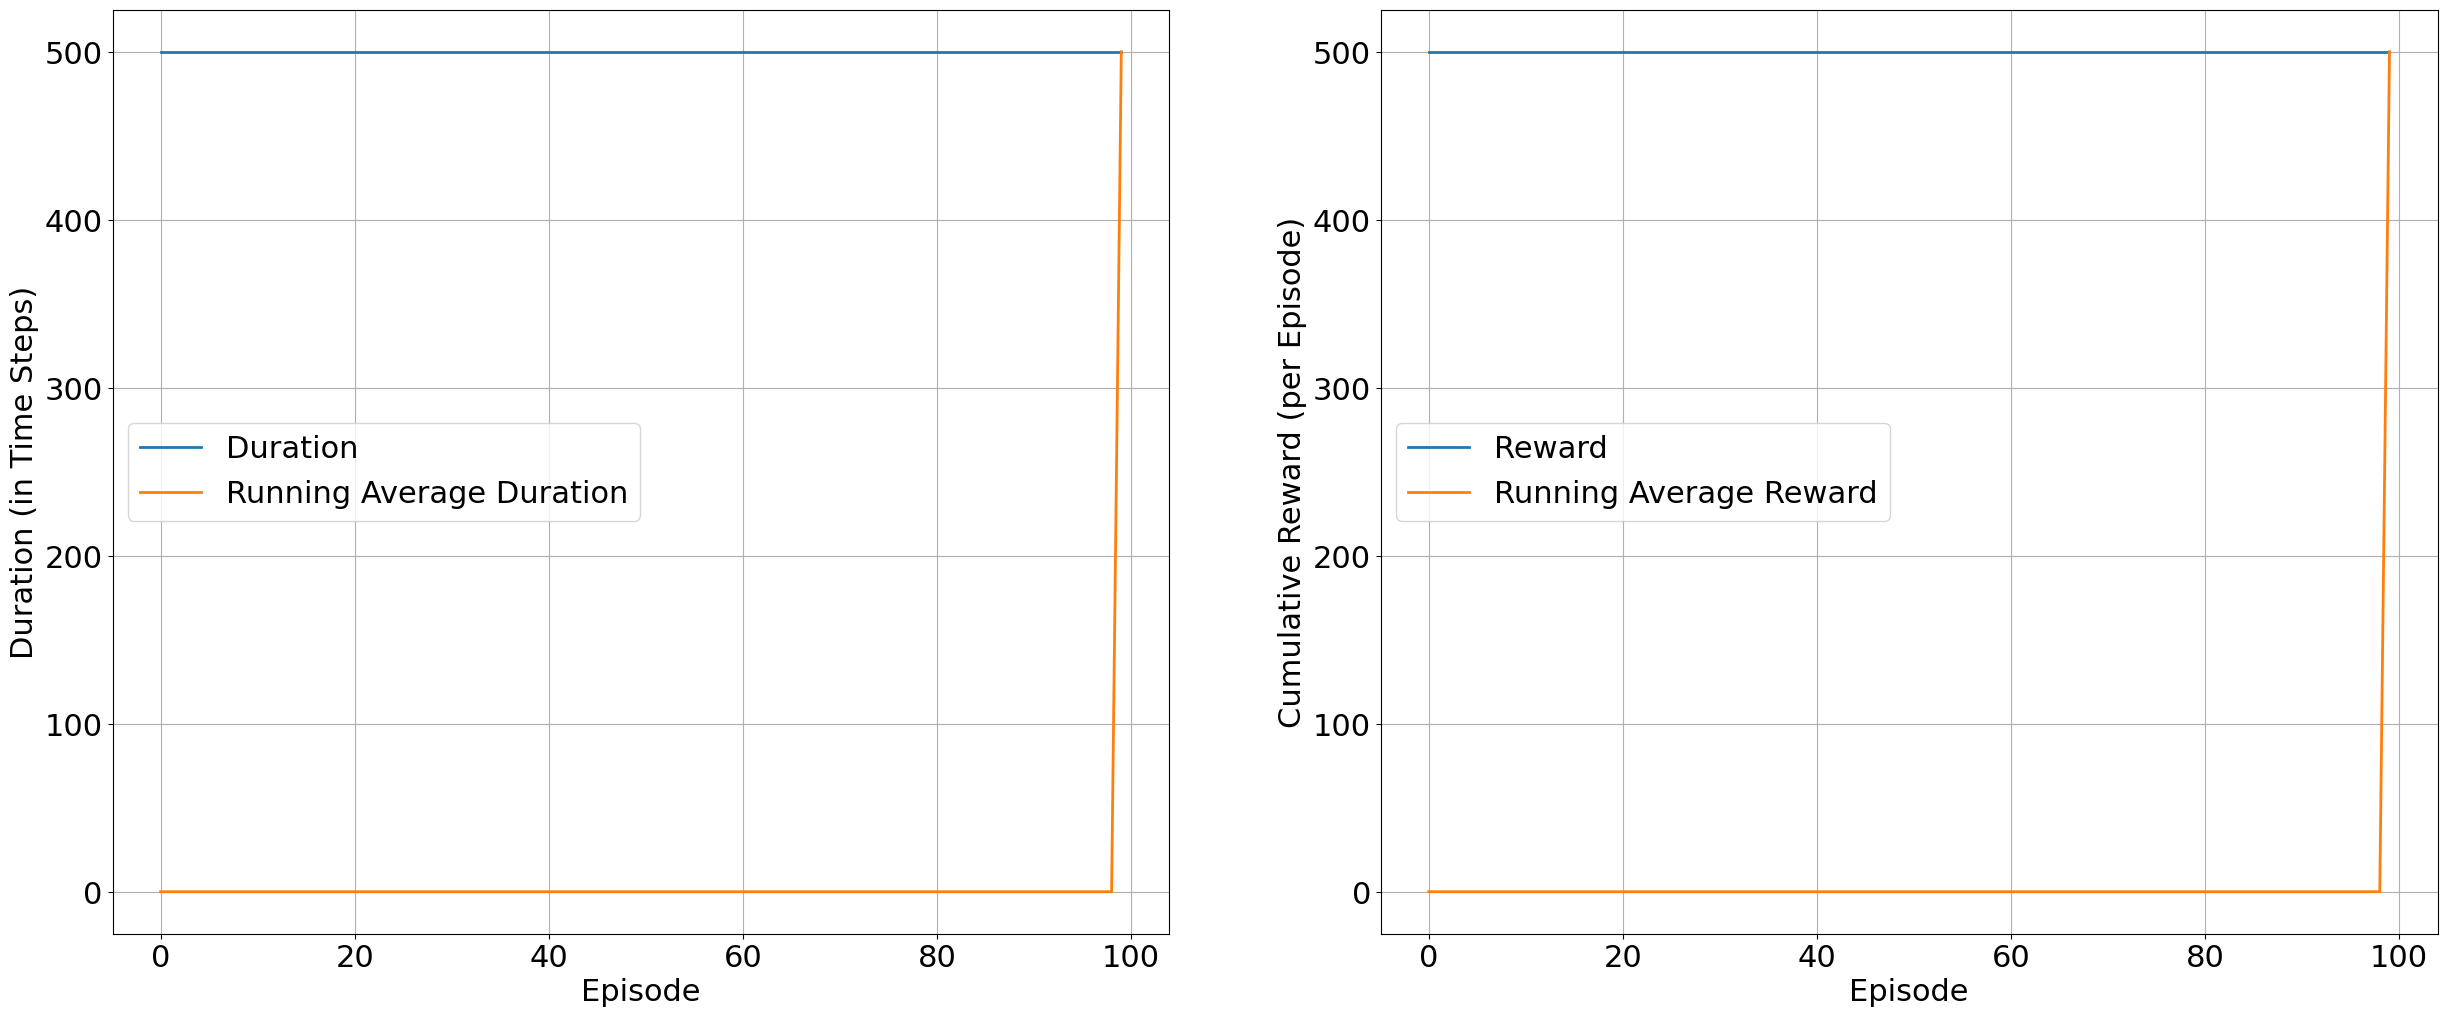
\includegraphics[width=\textwidth]{cart_evaluate.png}
    \end{center}
    \caption{Cart Environment Evaluation}
\end{figure}

\begin{figure}[H]
    \begin{center}
        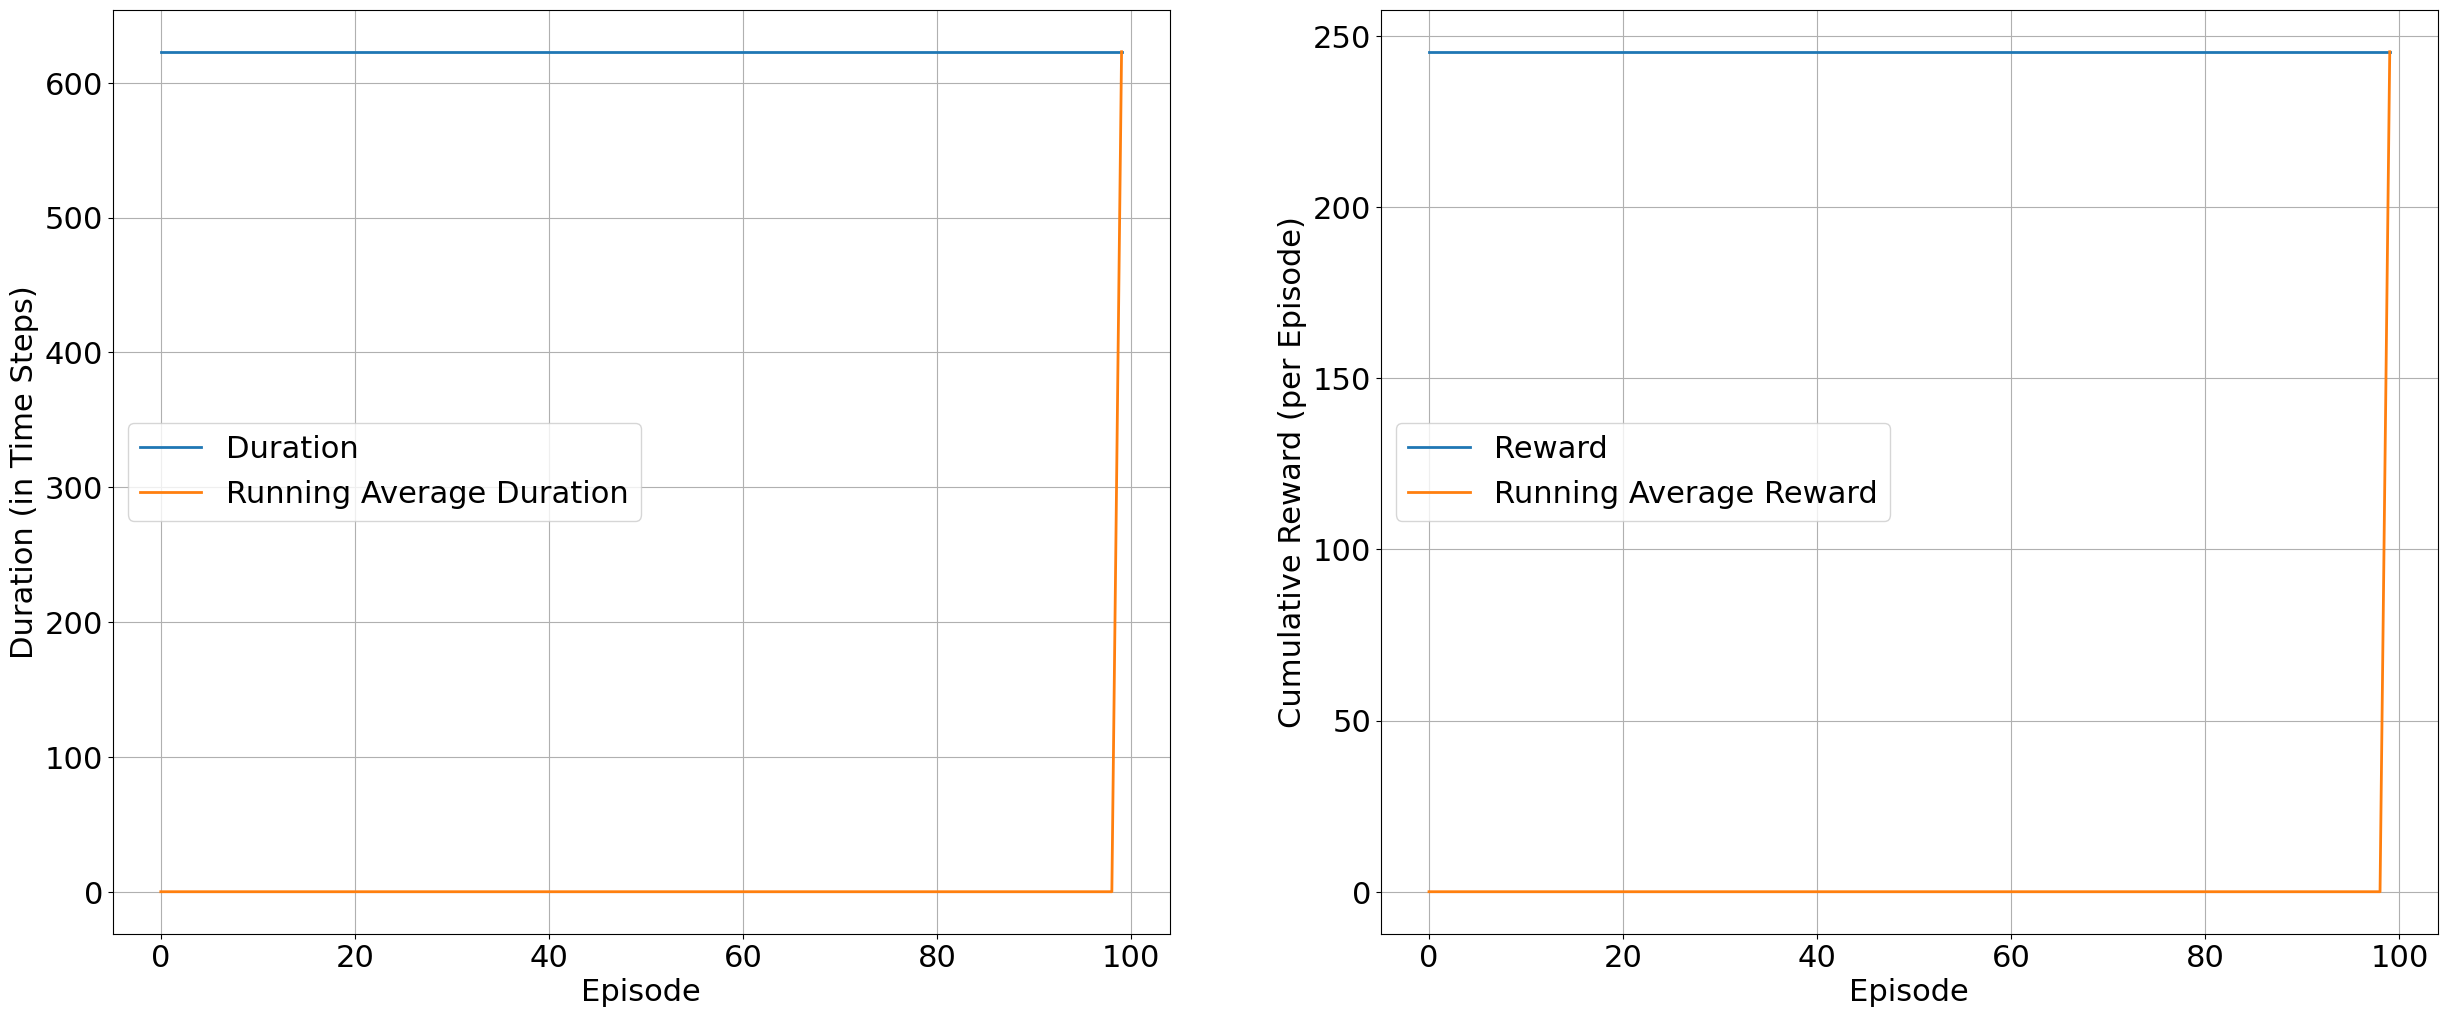
\includegraphics[width=\textwidth]{lunar_evaluate_ddqn.png}
    \end{center}
    \caption{Lunar Environment Evaluation}
\end{figure}

The Double Q-Learning with a \verb|FeedForward| neural network approach has successfully learned the optimal
policy for all three environments. The evaluation result for the GridEnvironment varies
due to the agent being placed at a random start squares, which affect the number of steps
required to reach the goal. To encourage the agent to reach the goal as quickly as possible,
we applied a negative reward of $-0.1$ for each step taken.

\section{Training Strategy Comparison}

\subsection{GridWorld}

\begin{figure}[H]
    \begin{center}
        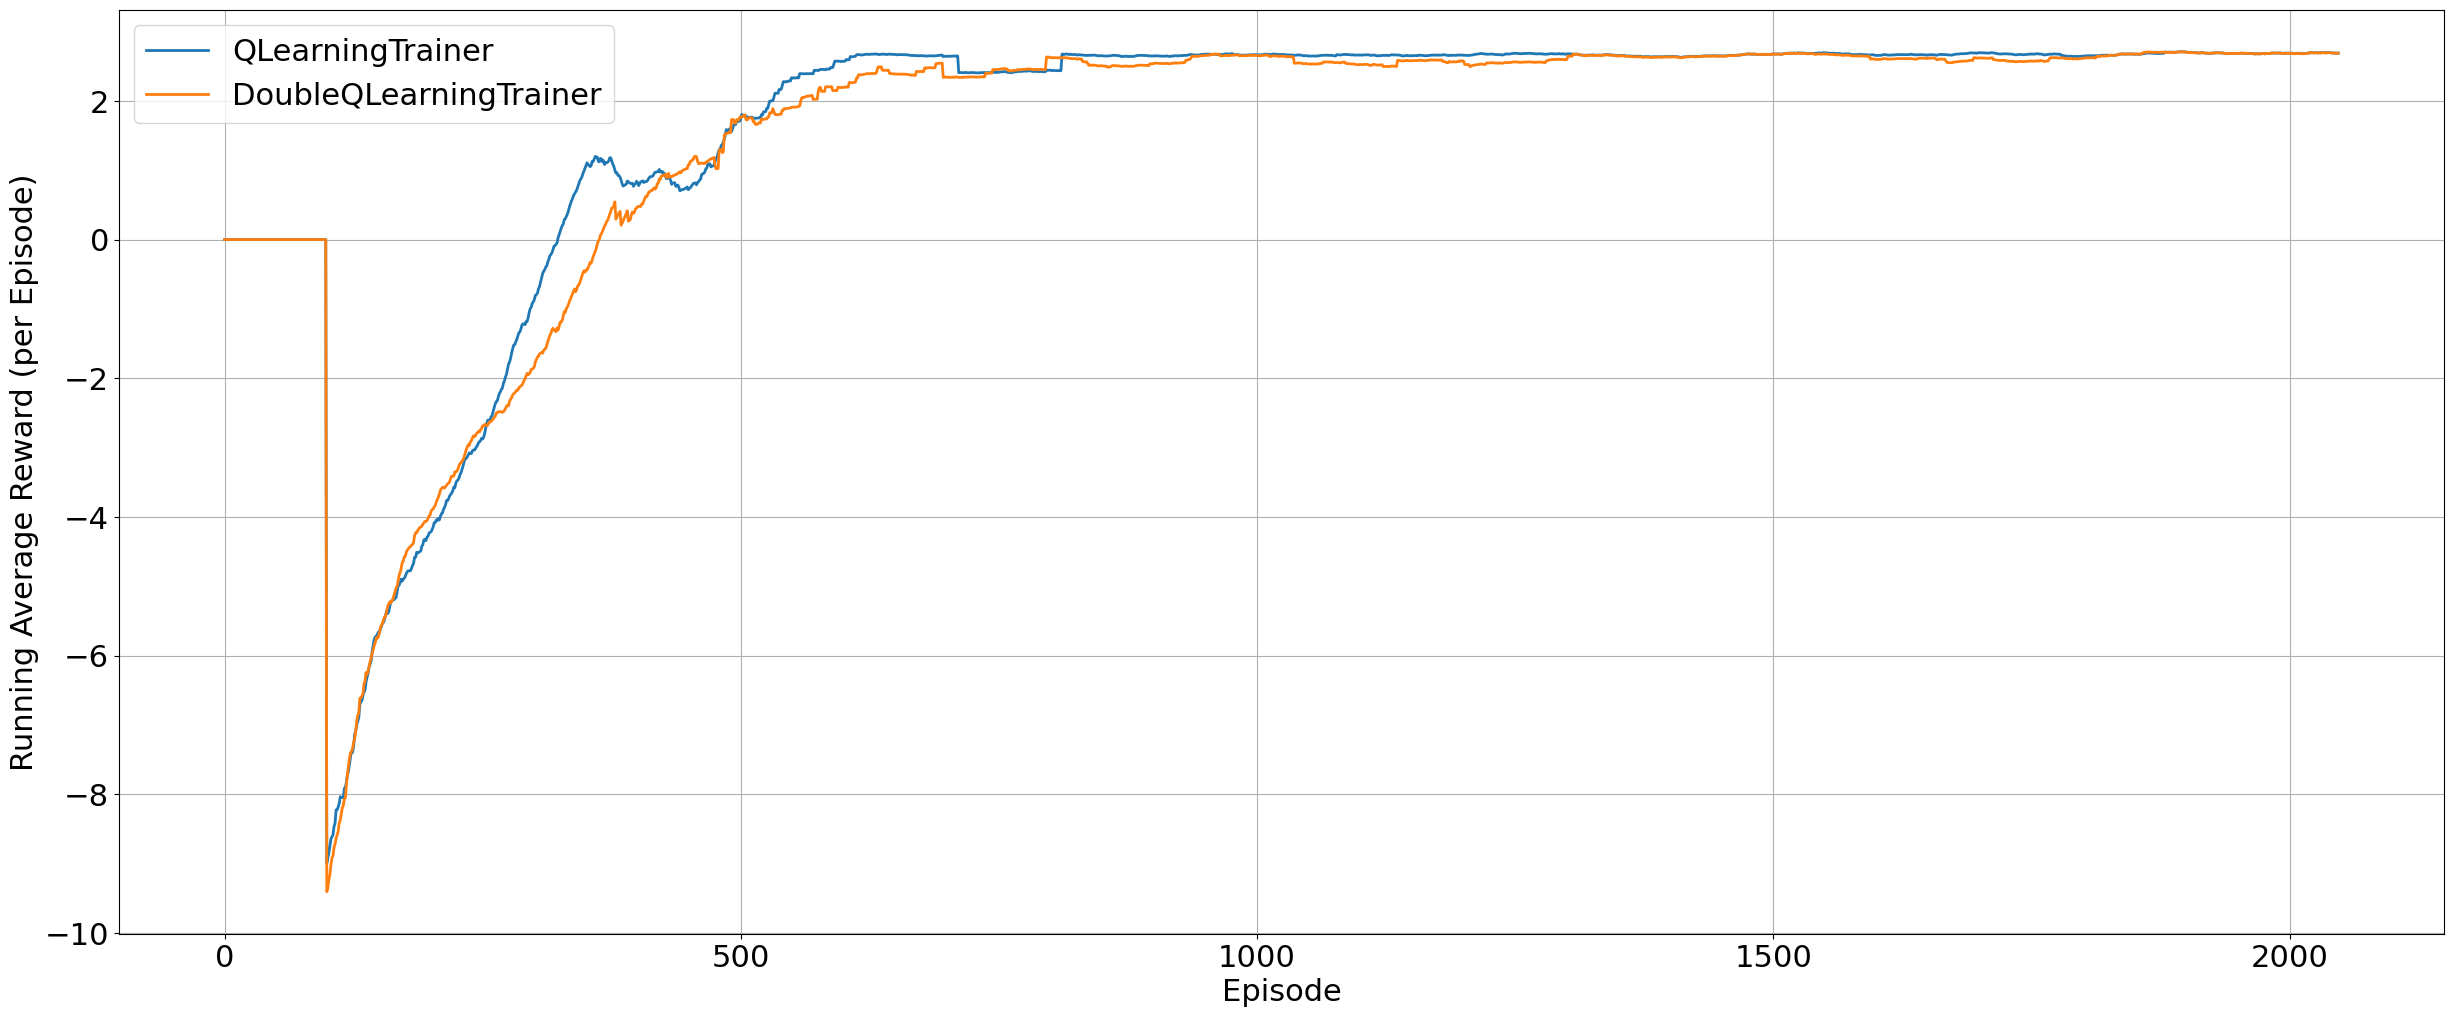
\includegraphics[width=\textwidth]{grid_compare.png}
    \end{center}
    \caption{Gridworld Agent Training Comparison}
\end{figure}

The GridWorld environment is relatively simple, both the DQN and DDQN models may have enough capacity to learn the optimal solution. The capacity of a model refers to its ability to capture the complexities and patterns in the data. In more complex environments, the DDQN model may have an advantage over the DQN model since it can more effectively learn the optimal action values by reducing overestimation bias.

Secondly, since the GridWorld environment is not very complex, the exploration-exploitation trade-off is not a significant concern. Both the DQN and DDQN models can effectively explore the environment and learn the optimal solution without getting stuck in local minima.

Therefore, it is not surprising that the DQN and DDQN models converge at nearly similar rates in a simplistic environment like the GridWorld environment.

\subsection{Cartpole v-1}

\begin{figure}[H]
    \begin{center}
        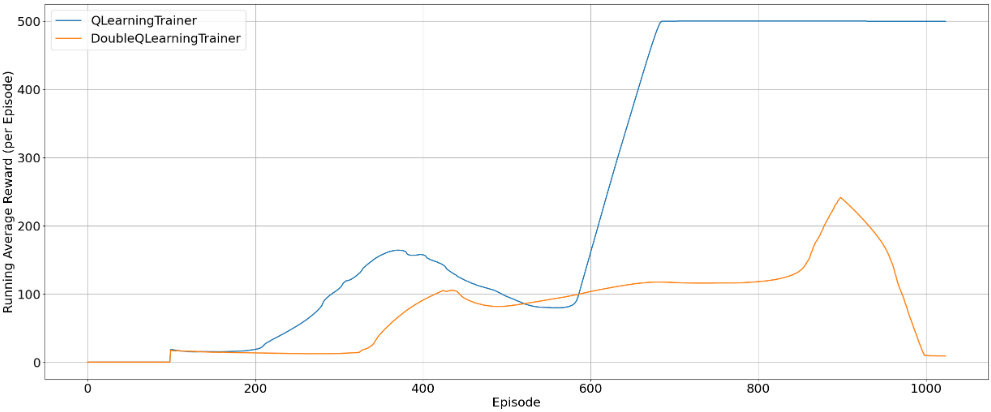
\includegraphics[width=\textwidth]{cart_compare.png}
    \end{center}
    \caption{LunarLander Agent Training Comparison}
\end{figure}

In some instances of this environment, the DQN model may outperform the DDQN model.

One reason for this could be that the DDQN model is highly sensitive to its hyperparameters, such as the learning rate and discount factor. Finding optimal hyperparameters for the DDQN model can be difficult, especially in more complex environments. In contrast, the DQN model may be more stable during training and may require less tuning of hyperparameters.

Overall, the DQN model may be a simpler and more stable choice for solving the CartPole environment, although the performance of both models can depend on the specific instance of the environment and the hyperparameters used.

\subsection{LunarLander v-2}

\begin{figure}[H]
    \begin{center}
        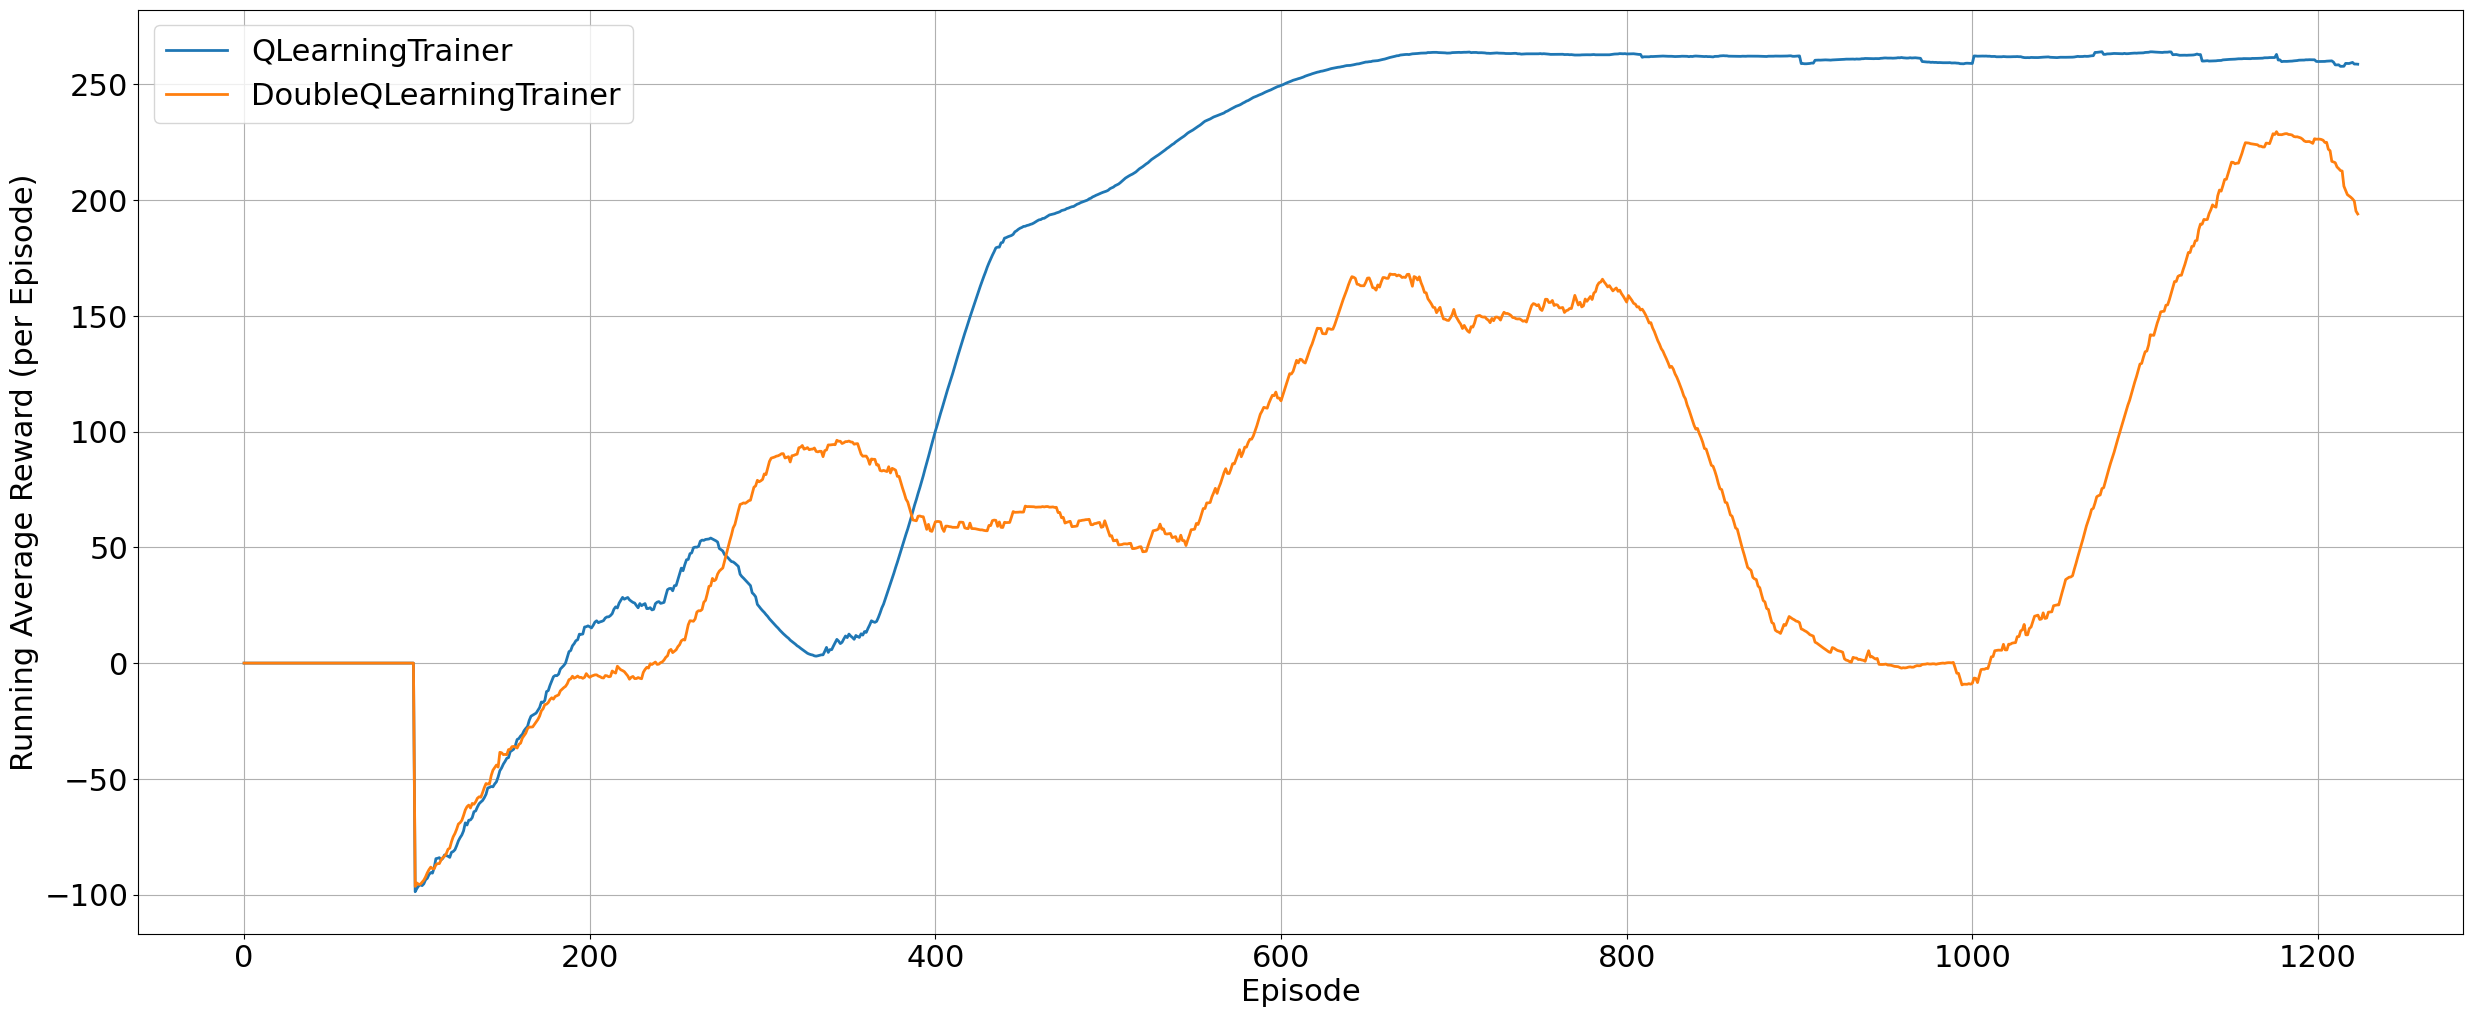
\includegraphics[width=\textwidth]{lunar_compare.png}
    \end{center}
    \caption{LunarLander Agent Training Comparison}
\end{figure}

The LunarLander v-2 is again rather simple in terms of it's state and action spaces. And we
see that the DQN slightly outperforms the DDQN algorithm. However, hyperparameters could be
a factor--the performance of both DQN and DDQN can be highly sensitive to their
hyperparameters, such as learning rate, batch size, and discount factor. It's possible that
the
hyperparameters used for the DQN algorithm were more suitable for the specific instance of
the LunarLander v2 environment (discrete), while the hyperparameters used for the DDQN algorithm were
not as optimal.

\printbibliography

\end{document}